% Malware Workshop
% Copyright (C) 2018  Lilly Chalupowski

% This program is free software: you can redistribute it and/or modify
% it under the terms of the GNU General Public License as published by
% the Free Software Foundation, either version 3 of the License, or
% (at your option) any later version.

% This program is distributed in the hope that it will be useful,
% but WITHOUT ANY WARRANTY; without even the implied warranty of
% MERCHANTABILITY or FITNESS FOR A PARTICULAR PURPOSE.  See the
% GNU General Public License for more details.

% You should have received a copy of the GNU General Public License
% along with this program.  If not, see <https://www.gnu.org/licenses/>.

\documentclass[aspectratio=169]{beamer}
\usepackage{tabularx}
\usepackage{graphicx}
\usepackage{eso-pic}
\usepackage{minted}
\usepackage{hyperref}
\usepackage{tcolorbox}

\makeatletter
\newenvironment{myitemize}{%
  \setlength{\topsep}{0pt}
  \setlength{\partopsep}{0pt}
  \renewcommand*{\@listi}{\leftmargin\leftmargini \parsep\z@ \topsep\z@ \itemsep\z@}
  \let\@listI\@listi
  \itemize
}{\enditemize}
\makeatother

\graphicspath{{img/}}

\usetheme{Warsaw}
\usemintedstyle{monokai}

\setbeamercolor{normal text}{fg=white,bg=black!90}
\setbeamercolor{structure}{fg=white}
\setbeamercolor{alerted text}{fg=red!85!black}
\setbeamercolor{item projected}{use=item,fg=black,bg=item.fg!35}
\setbeamercolor*{palette primary}{use=structure,fg=structure.fg}
\setbeamercolor*{palette secondary}{use=structure,fg=structure.fg!95!black}
\setbeamercolor*{palette tertiary}{use=structure,fg=structure.fg!90!black}
\setbeamercolor*{palette quaternary}{use=structure,fg=structure.fg!95!black,bg=black!80}
\setbeamercolor*{framesubtitle}{fg=white}
\setbeamercolor*{block title}{parent=structure,bg=black!60}
\setbeamercolor*{block body}{fg=black,bg=black!10}
\setbeamercolor*{block title alerted}{parent=alerted text,bg=black!15}
\setbeamercolor*{block title example}{parent=example text,bg=black!15}
\setbeamertemplate{navigation symbols}{}
\setbeamercolor{footercolor}{fg=white,bg=black}

\makeatletter
\defbeamertemplate*{footline}{myfootline}
{
  \leavevmode%
  \hbox{%
    \begin{beamercolorbox}[wd=.333333\paperwidth,ht=2.25ex,dp=1ex,center]{footercolor}%
      \insertshorttitle
    \end{beamercolorbox}%
    \begin{beamercolorbox}[wd=.333333\paperwidth,ht=2.25ex,dp=1ex,center]{footercolor}%
      \insertshortauthor\expandafter\beamer@ifempty\expandafter{\beamer@shortinstitute}{}{~~(\insertshortinstitute)}
    \end{beamercolorbox}%
    \begin{beamercolorbox}[wd=.333333\paperwidth,ht=2.25ex,dp=1ex,right]{footercolor}%
      \insertshortdate{}\hspace*{2em}
      \insertframenumber{} / \inserttotalframenumber\hspace*{2ex} 
    \end{beamercolorbox}}%
  \vskip0pt%
}
\makeatother

\title{Malware Unpacking Workshop}

\institute{GoSecure}
\author{Lilly Chalupowski}
\date{August 28, 2019}

\begin{document}

\setbeamertemplate{footline}{}
\begin{frame}[t]
  \begin{center}
    \begingroup
    \fontsize{20pt}{20pt}\selectfont
    \inserttitle \\
    \endgroup
    \bigskip
    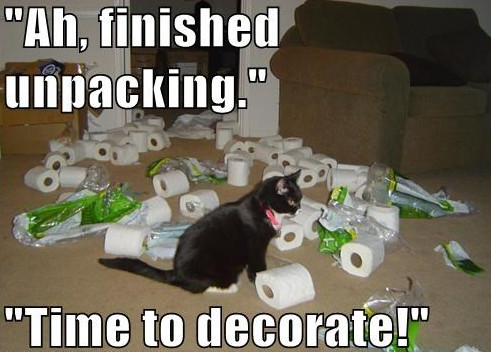
\includegraphics[scale=0.6]{unpacking-cat-meme} \\
    \bigskip
    \insertauthor \\
    \insertdate
  \end{center}
\end{frame}

\setbeamertemplate{footline}[myfootline]

\begin{frame}
  \frametitle{whois lilly.chalupowski}
  \begin{table}
    \caption{\textit{who.is results}}
    \begin{tabularx}{\textwidth}{|X|X|}
      \hline
      Name & Lilly Chalupowski \\
      \hline
      Status & Employed \\
      \hline
      Creation Date & 1986 \\
      \hline
      Expiry & A Long Time from Now (Hopefully)\\
      \hline
      Registrant Name & GoSecure \\
      \hline
      Administrative Contact & Travis Barlow \\
      \hline
      Job & TITAN Malware Research Lead \\
      \hline
    \end{tabularx}
  \end{table}
\end{frame}

\begin{frame}
  \frametitle{Agenda}
  \framesubtitle{What will we cover?}
  \begin{columns}[onlytextwidth]
    \begin{column}{.50\textwidth}
      \begin{itemize}
      \item{Disclaimer}
      \item{Reverse Engineering}
      \item{Tools of the Trade}
      \item{Injection Techniques}
      \item{Workshop}
      \end{itemize}
    \end{column}
    \hfill
    \begin{column}{.50\textwidth}
      \begin{center}
        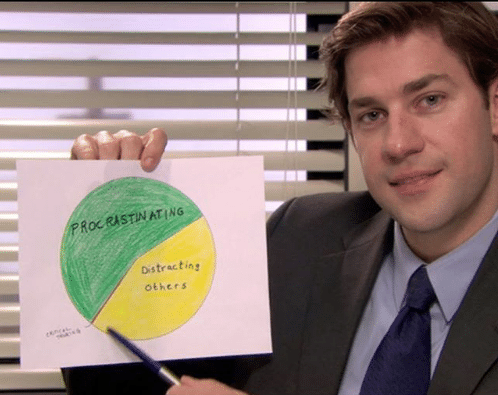
\includegraphics[scale=1.8]{agenda-meme}
      \end{center}
    \end{column}
  \end{columns}
\end{frame}

\begin{frame}
  \frametitle{Disclaimer}
  \framesubtitle{Don't be a Criminal}
  \begin{tcolorbox}[title=disclaimer\_0.log,colback=gray]
    The tools and techniques covered in this presentation can be dangerous and are\\
    being shown for educational purposes.\\
    \newline
    It is a violation of Federal laws to attempt gaining unauthorized access to information, assets or systems belonging to others, or to exceed authorization on systems for which you have not been granted.\\
    \newline
    Only use these tools with/on systems you own or have written permission from the owner. I (the speaker) do not assume any responsibility and shall not be held liable for any illegal use of these tools.\\
  \end{tcolorbox}
\end{frame}

\begin{frame}
  \frametitle{Disclaimer}
  \framesubtitle{Don't be a Fool}
  \begin{tcolorbox}[title=disclaimer\_1.log,colback=gray]
    I (the speaker) do not assume any responsibility and shall not be held
    liable for anyone who infects their machine with the malware supplied for
    this workshop. \\
    \newline
    If you need help on preventing the infection of your host machine please
    raise your hand during the workshop for assistance before you run anything. \\
    \newline
    The malware used in this workshop can steal your data, shutdown nuclear
    power plants, encrypt your files and more. \\
  \end{tcolorbox}
\end{frame}

\begin{frame}
  \frametitle{Reverse Engineering}
  \begin{center}
    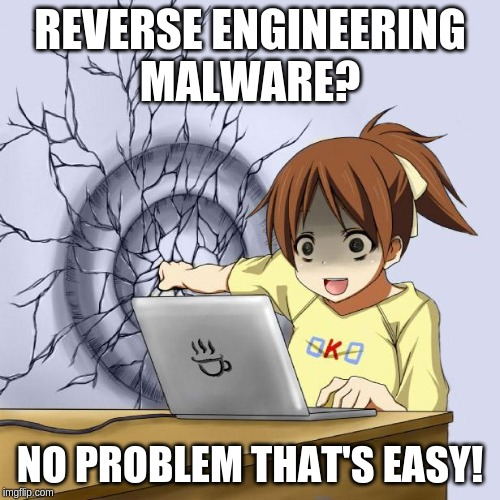
\includegraphics[scale=0.4]{reverse-engineering}
  \end{center}
\end{frame}

\begin{frame}
  \frametitle{Registers}
  \framesubtitle{reverse\_engineering: 0x00}
  \begin{columns}
    \begin{column}{.50\textwidth}
      \begin{itemize}
      \item{EAX - Return Value of Functions}
      \item{EBX - Base Index (for use with arrays)}
      \item{ECX - Counter in Loops}
      \item{EDI - Destination Memory Operations}
      \item{ESI - Source Memory Operations}
      \item{ESP - Stack Pointer}
      \item{EBP - Base Frame Pointer}
      \end{itemize}
    \end{column}
    \hfill
    \begin{column}{.50\textwidth}
      \begin{center}
        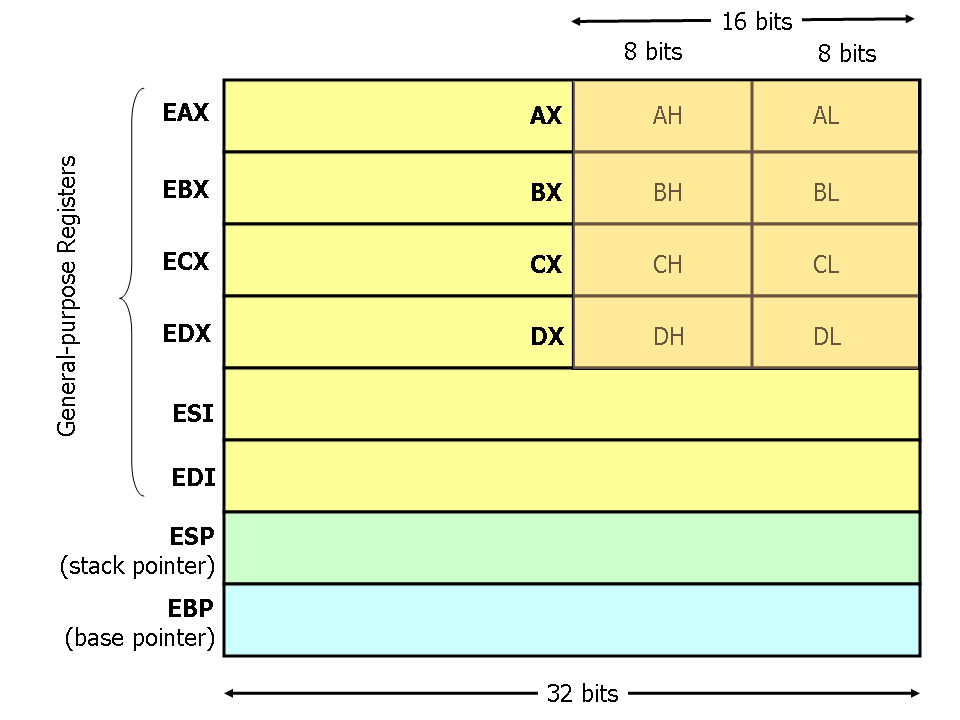
\includegraphics[scale=0.25]{x86-registers}
      \end{center}
    \end{column}
  \end{columns}
  \bigskip
  Did You Know: In computer architecture, a processor register is a quickly accessible location available to a computer's central processing unit (CPU).
\end{frame}

\begin{frame}
  \frametitle{Registers}
  \framesubtitle{reverse\_engineering: 0x01}
  \begin{center}
    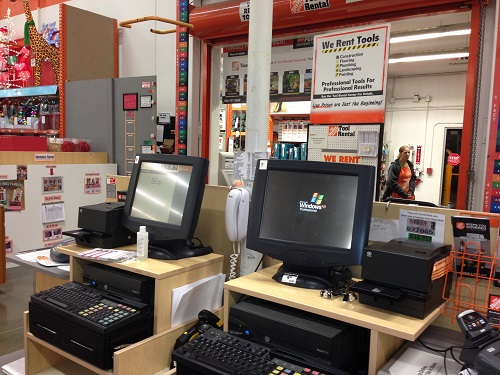
\includegraphics[scale=0.5]{cash-register}
  \end{center}
\end{frame}

\begin{frame}
  \frametitle{Stack Overview}
  \framesubtitle{reverse\_engineering: 0x02}
  \begin{columns}
    \begin{column}{.40\textwidth}
      \begin{itemize}
      \item{Last-In First-Out}
      \item{Downward Growth}
      \item{Function Local Variables}
      \item{ESP}
      \item{Increment / Decrement = 4}
        \begin{itemize}
        \item{Double-Word Aligned}
        \end{itemize}
      \end{itemize}
    \end{column}
    \hfill
    \begin{column}{.60\textwidth}
      \begin{center}
        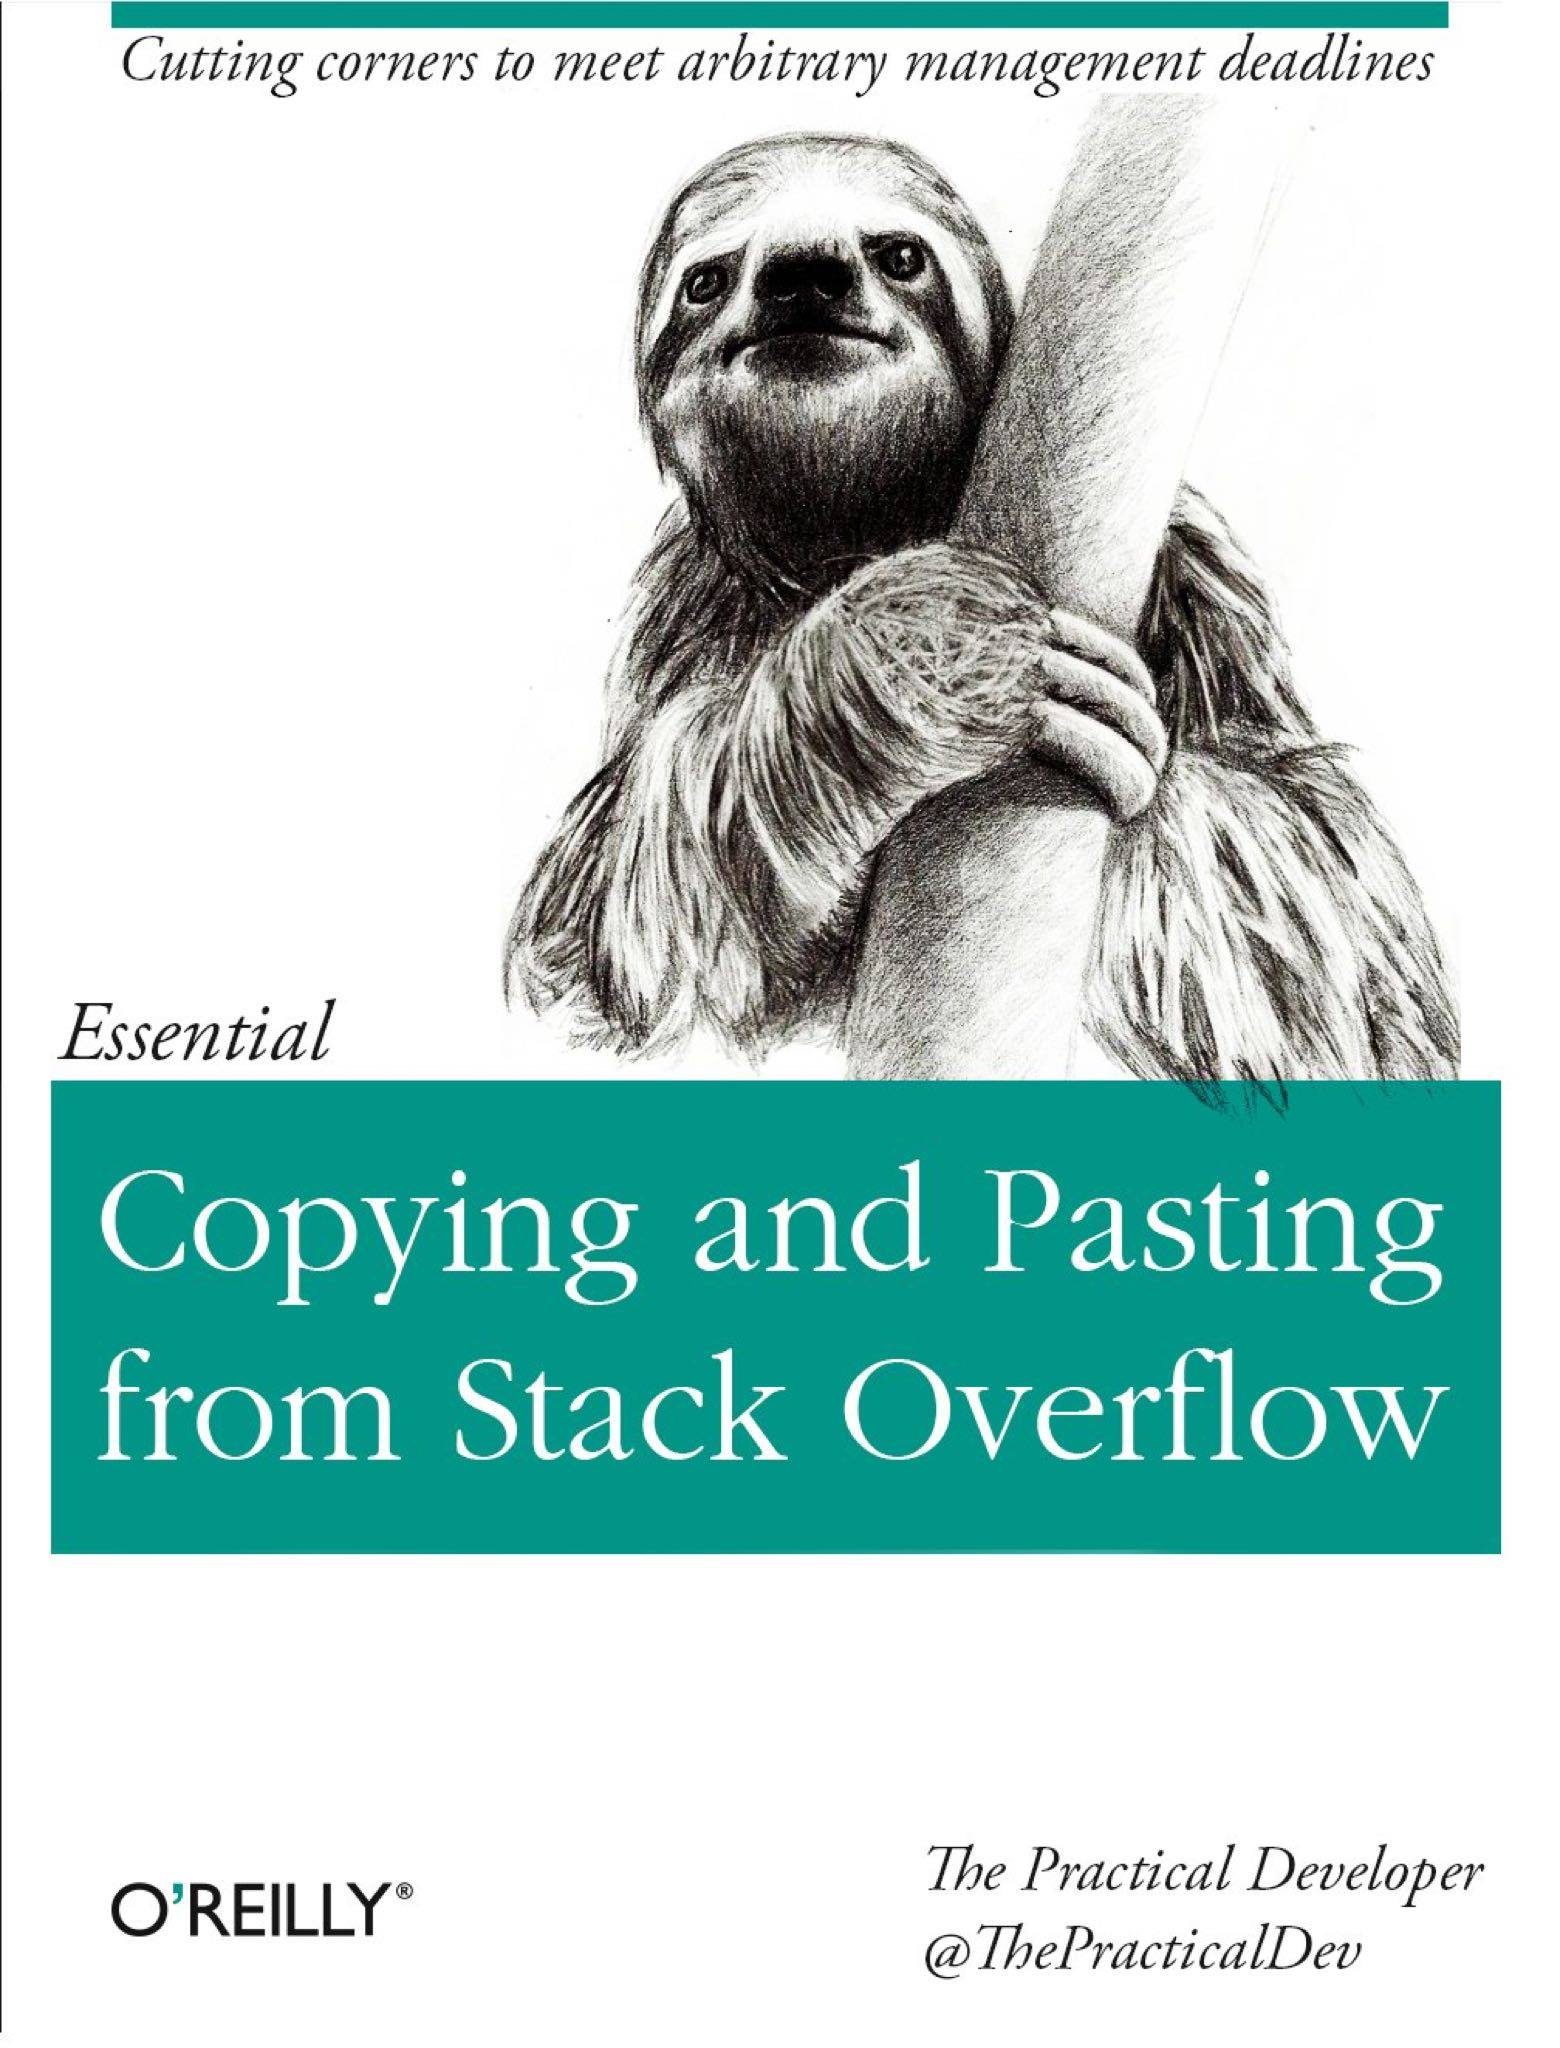
\includegraphics[scale=0.09]{stack-overflow-meme}
      \end{center}
    \end{column}
  \end{columns}
  \end{frame}

\begin{frame}
  \frametitle{Stack Structure}
  \framesubtitle{reverse\_engineering: 0x03}
  \begin{center}
    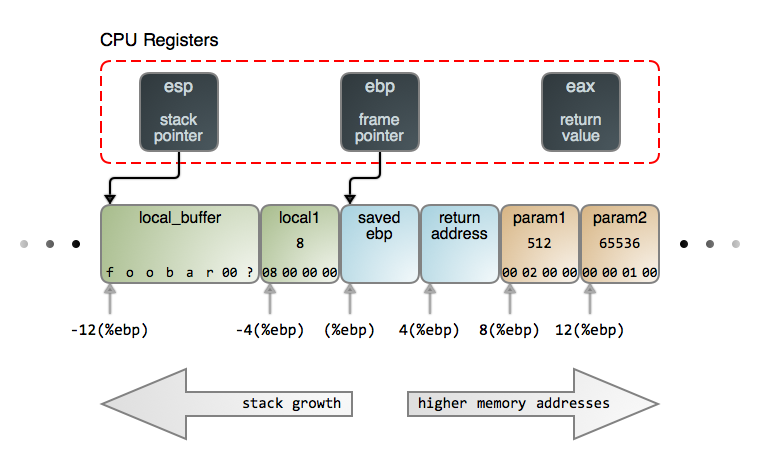
\includegraphics[scale=0.42]{the-stack}
  \end{center}
\end{frame}

\begin{frame}
  \frametitle{Control Flow}
  \framesubtitle{reverse\_engineering: 0x04}
  \begin{columns}
    \begin{column}{.5\textwidth}
      \begin{itemize}
        \item{Conditionals}
          \begin{itemize}
          \item{CMP}
            % Compares both operands by subtraction to determine if the result
            % is 0
          \item{TEST}
           % [TEST] computes the bit-wise logical AND of first operand (source 1 operand) and the second operand (source 2 operand) and sets the SF, ZF, and PF status flags according to the result. 
           % A	 	B	 	C
           % 0	 AND 	0	->	0
           % 0	 AND 	1	->	0
           % 1	 AND 	0	->	0
           % 1	 AND 	1	->	1
          \item{JMP}
          % Jumps to the specified address
          \item{JNE}
          \item{JNZ}
          \end{itemize}
      \item{EFLAGS}
        \begin{itemize}
        \item{ZF / Zero Flag}
          % Set if the result of the previous arithmetic operation is zero
        \item{SF / Sign Flag}
          % Set to the most significant bit of the result
          % Alternatively referred to as the alt bit, high bit, meta bit, or senior bit the most significant bit is the highest bit in a series of numbers in binary, located at the far left of a string. For example, in the number 01001001, the most significant bit is the 0 at the beginning of the line.
        \item{CF / Cary Flag}
          % Set when the result requires a carry. It applies to unsigned numbers
        \item{OF/Overflow Flag}
          % Set if the result overflows the max size. It applies to signed numbers
        \end{itemize}
      \end{itemize}
    \end{column}
    \hfill
    \begin{column}{.5\textwidth}
      \begin{center}
        
\includegraphics[scale=0.25]{zero-flag-meme}
      \end{center}
    \end{column}
  \end{columns}
\end{frame}

\begin{frame}
  \frametitle{Calling Conventions}
  \framesubtitle{reverse\_engineering: 0x05}
  \begin{columns}
    \begin{column}{.5\textwidth}
      \begin{itemize}
      \item{CDECL}
        \begin{itemize}
        \item{Arguments Right-to-Left}
        \item{Return Values in EAX}
        \item{Calling Function Cleans the Stack}
        \end{itemize}
      \item{STDCALL}
        \begin{itemize}
        \item{Used in Windows Win32API}
        \item{Arguments Right-to-Left}
        \item{Return Values in EAX}
        \item{The called function cleans the stack, unlike CDECL}
        \item{Does not support variable arguments}
        \end{itemize}
      \item{FASTCALL}
        \begin{itemize}
        \item{Uses registers as arguments}
        \item{Useful for shellcode}
        \end{itemize}
      \end{itemize}
    \end{column}
    \hfill
    \begin{column}{.5\textwidth}
      \begin{center}
        
\includegraphics[scale=0.27]{cdecl-meme}
      \end{center}
    \end{column}
  \end{columns}
\end{frame}

\begin{frame}
  \frametitle{Windows Memory Structure}
  \framesubtitle{reverse\_engineering: 0x06}
  \begin{columns}
    \begin{column}{.6\textwidth}
      \begin{itemize}
      \item{Stack - Grows up to lower addresses}
      \item{Heap - Grows down to higher addresses}
      \item{Program Image}
      \item{TEB - Thread Environment Block}
        \begin{itemize}
        \item{GetLastError()}
        \item{GetVersion()}
        \item{Pointer to the PEB}
        \end{itemize}
        % stores information about the currently running thread
        % The TIB can be used to get a lot of information on the process without calling Win32 API. Examples include emulating GetLastError(), GetVersion(). Through the pointer to the PEB one can obtain access to the import tables (IAT), process startup arguments, image name, etc. It is accessed from the FS segment register when operating on 32 bits, and from GS in 64 bits.
      \item{PEB - Process Environment Block}
        \begin{itemize}
        \item{Image Name}
        \item{Global Context}
        \item{Startup Parameters}
        \item{Image Base Address}
        \item{IAT (Import Address Table)}
        \end{itemize}
        % The PEB contains data structures that apply across a whole process, including global context, startup parameters, data structures for the program image loader, the program image base address, and synchronization objects used to provide mutual exclusion for process-wide data structures. 
      \end{itemize}
    \end{column}
    \hfill
    \begin{column}{.7\textwidth}
      \begin{center}
        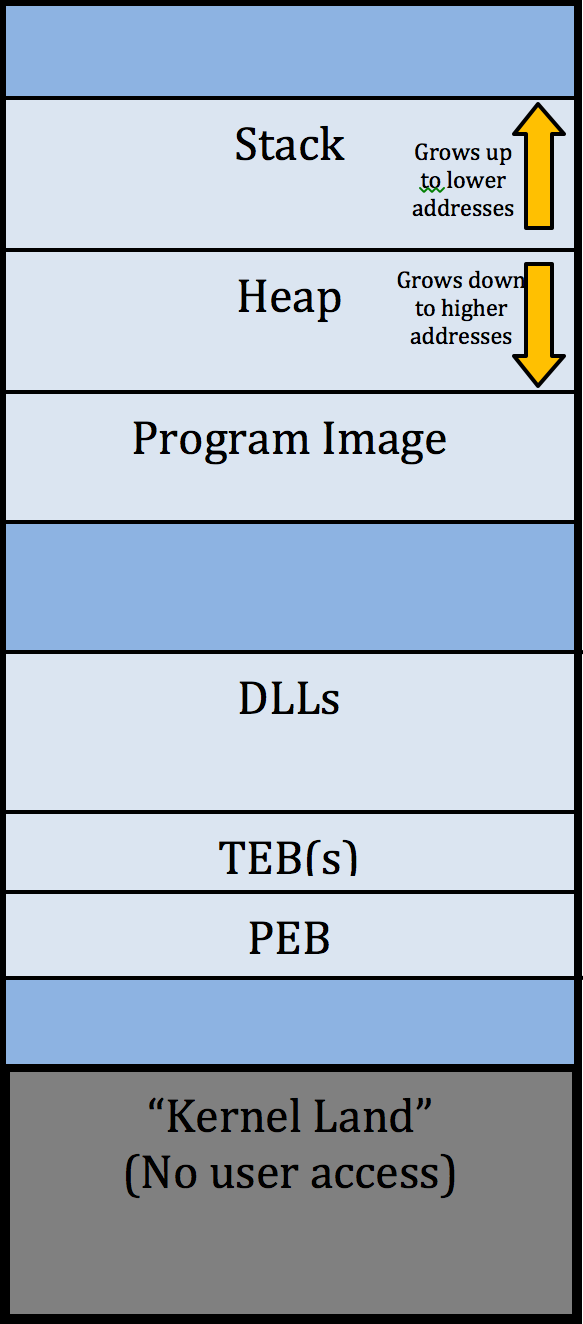
\includegraphics[scale=0.30]{the-heap}
      \end{center}
    \end{column}
  \end{columns}
\end{frame}

\begin{frame}
  \frametitle{IAT (Import Address Table) and IDT (Import Directory Table)}
  \framesubtitle{reverse\_engineering: 0x07}
  \begin{columns}
    \begin{column}{.4\textwidth}
      \begin{itemize}
        \item{Identical to the IDT (Import Directory Table)}
        \item{Binding - The process of where functions are mapped to their
            virtual addresses overwriting the IAT}
        \item{Often the IDT and IAT must be rebuilt when packing and unpacking malware}
      \end{itemize}
    \end{column}
    \hfill
    \begin{column}{.6\textwidth}
      \begin{center}
        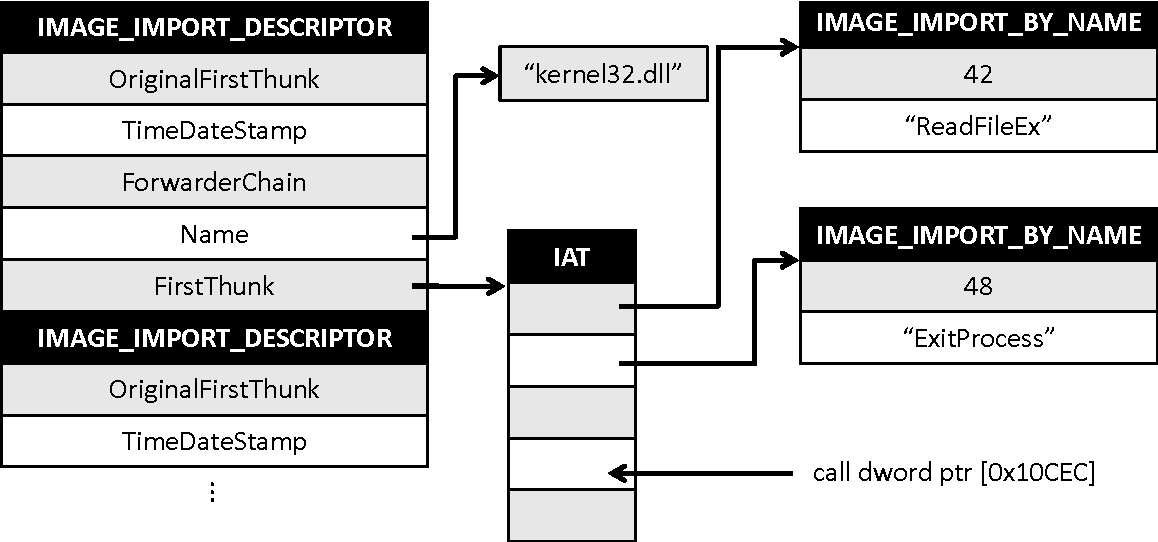
\includegraphics[scale=0.2]{IAT}
      \end{center}
    \end{column}
  \end{columns}
  % Mapped format is when it's mapped to memory with virtual addresses
  % after loaded by Windows
  % Unmapped is when it uses it's raw addresses before it's loaded into memory
  % by Windows
\end{frame}

\begin{frame}
  \frametitle{Assembly}
  \framesubtitle{reverse\_engineering: 0x08}
  \begin{columns}
    \begin{column}{.35\textwidth}
      \begin{itemize}
      \item{Common Instructions}
        \begin{itemize}
        \item{MOV}
        \item{LEA}
        \item{XOR}
        \item{PUSH}
        \item{POP}
      \end{itemize}
    \end{itemize}
    \end{column}
    \hfill
    \begin{column}{0.65\textwidth}
      \begin{center}
        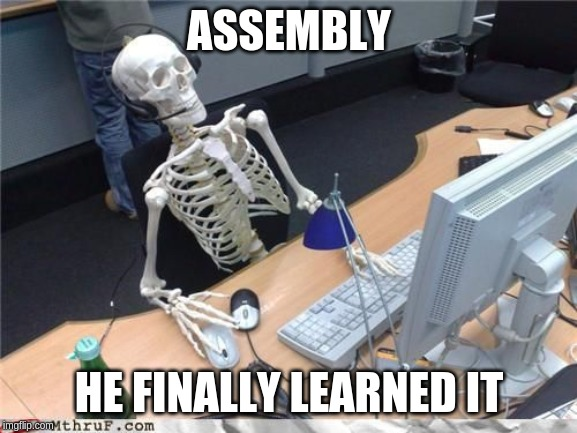
\includegraphics[scale=0.40]{assembly-meme}
      \end{center}
    \end{column}
  \end{columns}
\end{frame}

\begin{frame}[fragile]{}
  \frametitle{Assembly CDECL (Linux)}
  \framesubtitle{reverse\_engineering: 0x09}
  \begin{center}
    \begin{tcolorbox}[title=cdecl.c,colback=black]
        \begin{minted}[fontsize=\small]{c}
          __cdecl int add_cdecl(int a, int b){
            return a + b;
          }
          int x = add_cdecl(2, 3);
        \end{minted}
    \end{tcolorbox}
  \end{center}
\end{frame}

\begin{frame}[fragile]{}
  \frametitle{Assembly CDECL (Linux)}
  \framesubtitle{reverse\_engineering: 0x0a}
  \begin{center}
    \begin{tcolorbox}[title=cdecl.asm,colback=black]
        \begin{minted}[fontsize=\small]{asm}
          _add_cdecl:
            push ebp
            mov ebp, esp
            mov eax, [ebp + 8]  ; get 3 from the stack
            mov edx, [ebp + 12] ; get 2 from the stack
            add eax, edx        ; add values to eax
            pop ebp
            ret
          _start:
            push 3              ; second argument 
            push 2              ; first argument
            call _add_cdecl
            add esp, 8
        \end{minted}
    \end{tcolorbox}
  \end{center}
\end{frame}

\begin{frame}[fragile]{}
  \frametitle{Assembly STDCALL (Windows)}
  \framesubtitle{reverse\_engineering: 0x0b}
  \begin{center}
    \begin{tcolorbox}[title=stdcall.c,colback=black]
        \begin{minted}[fontsize=\small]{c}
          __stdcall int add_stdcall(int a, int b){
            return a + b;
          }
          int x = add_stdcall(2, 3);
        \end{minted}
    \end{tcolorbox}
  \end{center}
\end{frame}

\begin{frame}[fragile]{}
  \frametitle{Assembly STDCALL (Windows)}
  \framesubtitle{reverse\_engineering: 0x0c}
  \begin{center}
    \begin{tcolorbox}[title=stdcall.asm,colback=black]
        \begin{minted}[fontsize=\small]{asm}
          _add_stdcall:
            push ebp
            mov ebp, esp
            mov eax, [ebp + 8]  ; set eax to 3
            mov edx, [ebp + 12] ; set edx to 2
            add eax, edx
            pop ebp
            ret 8               ; how many bytes to pop
          _start:               ; main function
            push 3              ; second argument
            push 2              ; first argument
            call _add_stdcall
        \end{minted}
        % In the function body, the ret instruction has an (optional) argument that indicates how many bytes to pop off the stack when the function returns.
        % STDCALL functions are name-decorated with a leading underscore, followed by an @, and then the number (in bytes) of arguments passed on the stack. This number will always be a multiple of 4, on a 32-bit aligned machine.
    \end{tcolorbox}
  \end{center}
\end{frame}

\begin{frame}[fragile]{}
  \frametitle{Assembly FASTCALL}
  \framesubtitle{reverse\_engineering: 0x0d}
  \begin{center}
    \begin{tcolorbox}[title=cdecl.c,colback=black]
        \begin{minted}[fontsize=\small]{c}
          __fastcall int add_fastcall(int a, int b){
            return a + b;
          }
          int x = add_fastcall(2, 3);
        \end{minted}
        % The FASTCALL calling convention is not completely standard across all compilers, so it should be used with caution. In FASTCALL, the first 2 or 3 32-bit (or smaller) arguments are passed in registers, with the most commonly used registers being edx, eax, and ecx. Additional arguments, or arguments larger than 4-bytes are passed on the stack, often in Right-to-Left order (similar to CDECL). The calling function most frequently is responsible for cleaning the stack, if needed.
        % Because of the ambiguities, it is recommended that FASTCALL be used only in situations with 1, 2, or 3 32-bit arguments, where speed is essential.
    \end{tcolorbox}
  \end{center}
\end{frame}

\begin{frame}[fragile]{}
  \frametitle{Assembly FASTCALL}
  \framesubtitle{reverse\_engineering: 0x0e}
  \begin{center}
    \begin{tcolorbox}[title=fastcall.asm,colback=black]
        \begin{minted}[fontsize=\small]{asm}
          _add_fastcall:
            push ebp
            mov ebp, esp
            add eax, edx        ; add and save result in eax
            pop ebp
            ret
          _start:
            mov eax, 2          ; first argument
            mov edx, 3          ; second argument
            call _add_fastcall
        \end{minted}
        % In the function body, the ret instruction has an (optional) argument that indicates how many bytes to pop off the stack when the function returns.
        % STDCALL functions are name-decorated with a leading underscore, followed by an @, and then the number (in bytes) of arguments passed on the stack. This number will always be a multiple of 4, on a 32-bit aligned machine.
    \end{tcolorbox}
  \end{center}
\end{frame}


\begin{frame}[fragile]{}
  \frametitle{Guess the Calling Convention}
  \framesubtitle{reverse\_engineering: 0x0f}
  \begin{center}
    \begin{tcolorbox}[title=hello.asm,colback=black]
    \begin{minipage}{0.8\textwidth}
      \begin{minted}[fontsize=\small]{asm}
        section     .text                  ; the code section
        global      _start                 ; tell linker entrypoint
        _start:
          mov     edx,len                  ; message length
          mov     ecx,msg                  ; message to write
          mov     ebx,1                    ; file descriptor stdout
          mov     eax,4                    ; syscall number for write
          int     0x80                     ; linux x86 interrupt
          mov     eax,1                    ; syscall number for exit
          int     0x80                     ; linux x86 interrupt
        section     .data                  ; the data section
          msg     db  'Hello, world!',0x0  ; null terminated string
          len     equ \$ - msg             ; message length
      \end{minted}
    \end{minipage}
    \end{tcolorbox}
  \end{center}
\end{frame}

\begin{frame}
  \frametitle{Assembler and Linking}
  \framesubtitle{reverse\_engineering: 0x10}
  \begin{center}
    \begin{tcolorbox}[title=terminal,colback=black]
      \begin{minipage}{0.8\textwidth}
        \textbf{\textcolor{green}{malware@work \textcolor{blue}{\~ \$}}} \textcolor{white}{ nasm -f elf32 -o hello.o hello.asm}
        \newline
        \textbf{\textcolor{green}{malware@work \textcolor{blue}{\~ \$}}} \textcolor{white}{ ld -m elf\_i386 -o hello hello.o}
        \newline
        \textbf{\textcolor{green}{malware@work \textcolor{blue}{\~ \$}}} \textcolor{white}{ ./hello}
        \newline
        \textcolor{white}{ Hello, World!}
        \newline
        \textbf{\textcolor{green}{malware@work \textcolor{blue}{\~ \$}}}
      \end{minipage}
    \end{tcolorbox}
  \end{center}
\end{frame}

\begin{frame}
  \frametitle{Assembly Flavors}
  \framesubtitle{reverse\_engineering: 0x11}
  \begin{center}
    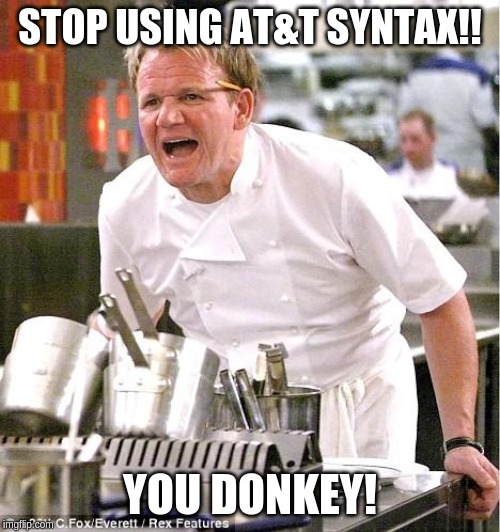
\includegraphics[scale=0.35]{intel-vs-atnt-meme}
  \end{center}
\end{frame}

\begin{frame}
  \frametitle{Tools of the Trade}
  \begin{center}
    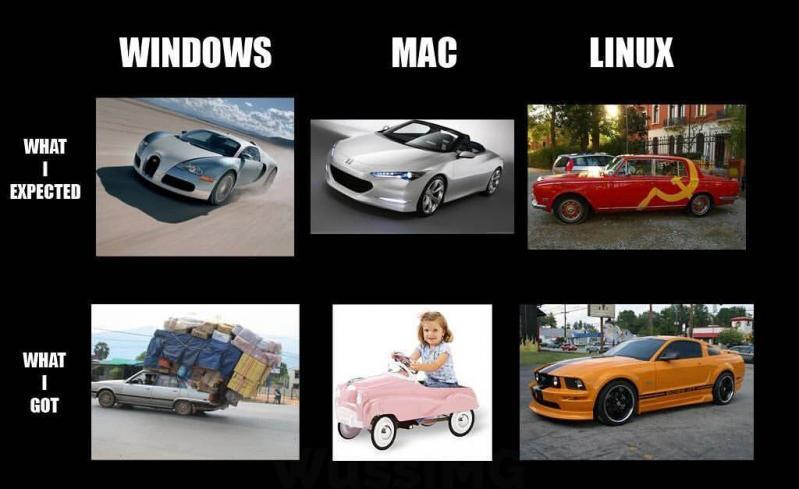
\includegraphics[scale=0.5]{mac-meme}
  \end{center}
\end{frame}

\begin{frame}
  \frametitle{VirtualBox}
  \framesubtitle{tools\_of\_the\_trade: 0x00}
  \begin{columns}
    \begin{column}{.3\textwidth}
      \begin{itemize}
      \item{Snapshots}
      \item{Security Layer}
      \item{Multiple Systems}
      \end{itemize}
    \end{column}
    \hfill
    \begin{column}{.7\textwidth}
      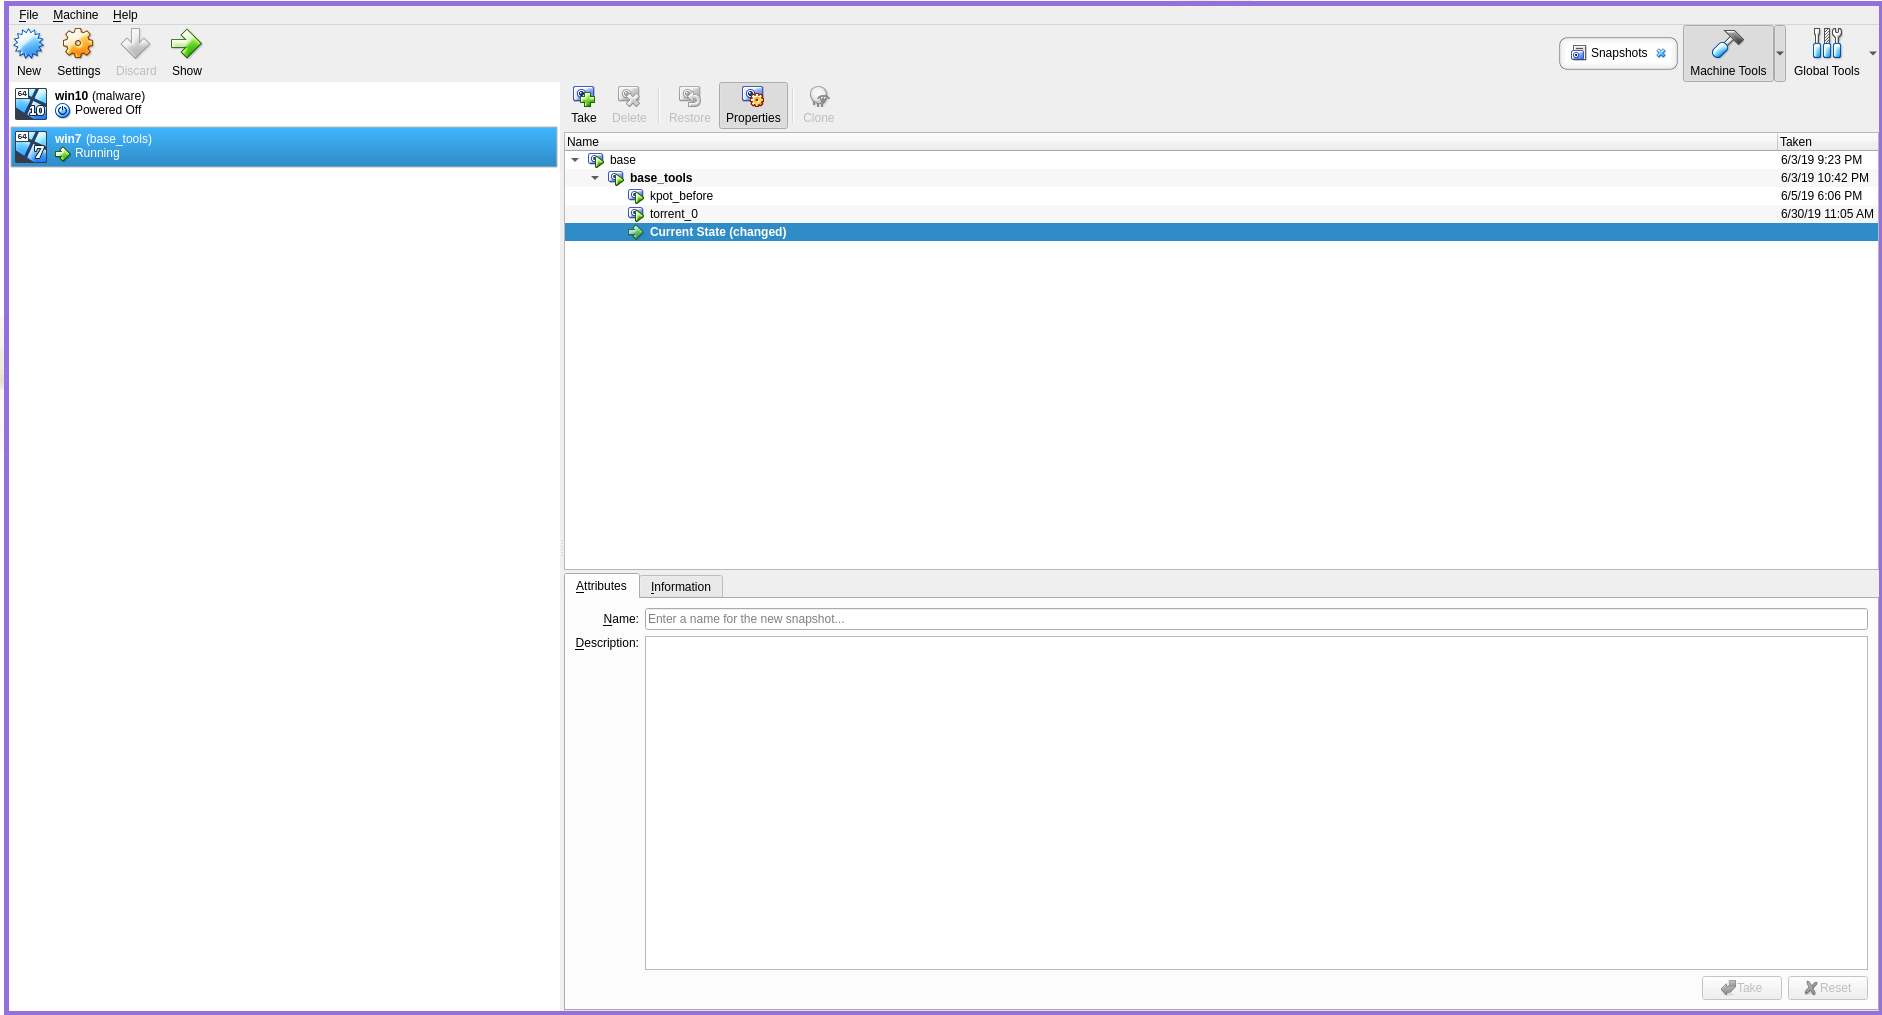
\includegraphics[scale=0.6]{virtualbox}
    \end{column}
  \end{columns}
\end{frame}

\begin{frame}
  \frametitle{x64dbg}
  \framesubtitle{tools\_of\_the\_trade: 0x01}
  \begin{columns}
    \begin{column}{.3\textwidth}
      \begin{itemize}
      \item{Resolving APIs}
      \item{Dumping Memory}
      \item{Modify Control Flow}
      \item{Identify Key Behaviors}
      \end{itemize}
    \end{column}
    \hfill
    \begin{column}{.7\textwidth}
      \begin{center}
        
\includegraphics[scale=0.5]{stages-of-debugging-meme}
      \end{center}
    \end{column}
  \end{columns}
\end{frame}

\begin{frame}
  \frametitle{x64dbg}
  \framesubtitle{tools\_of\_the\_trade: 0x02}
  \begin{center}
    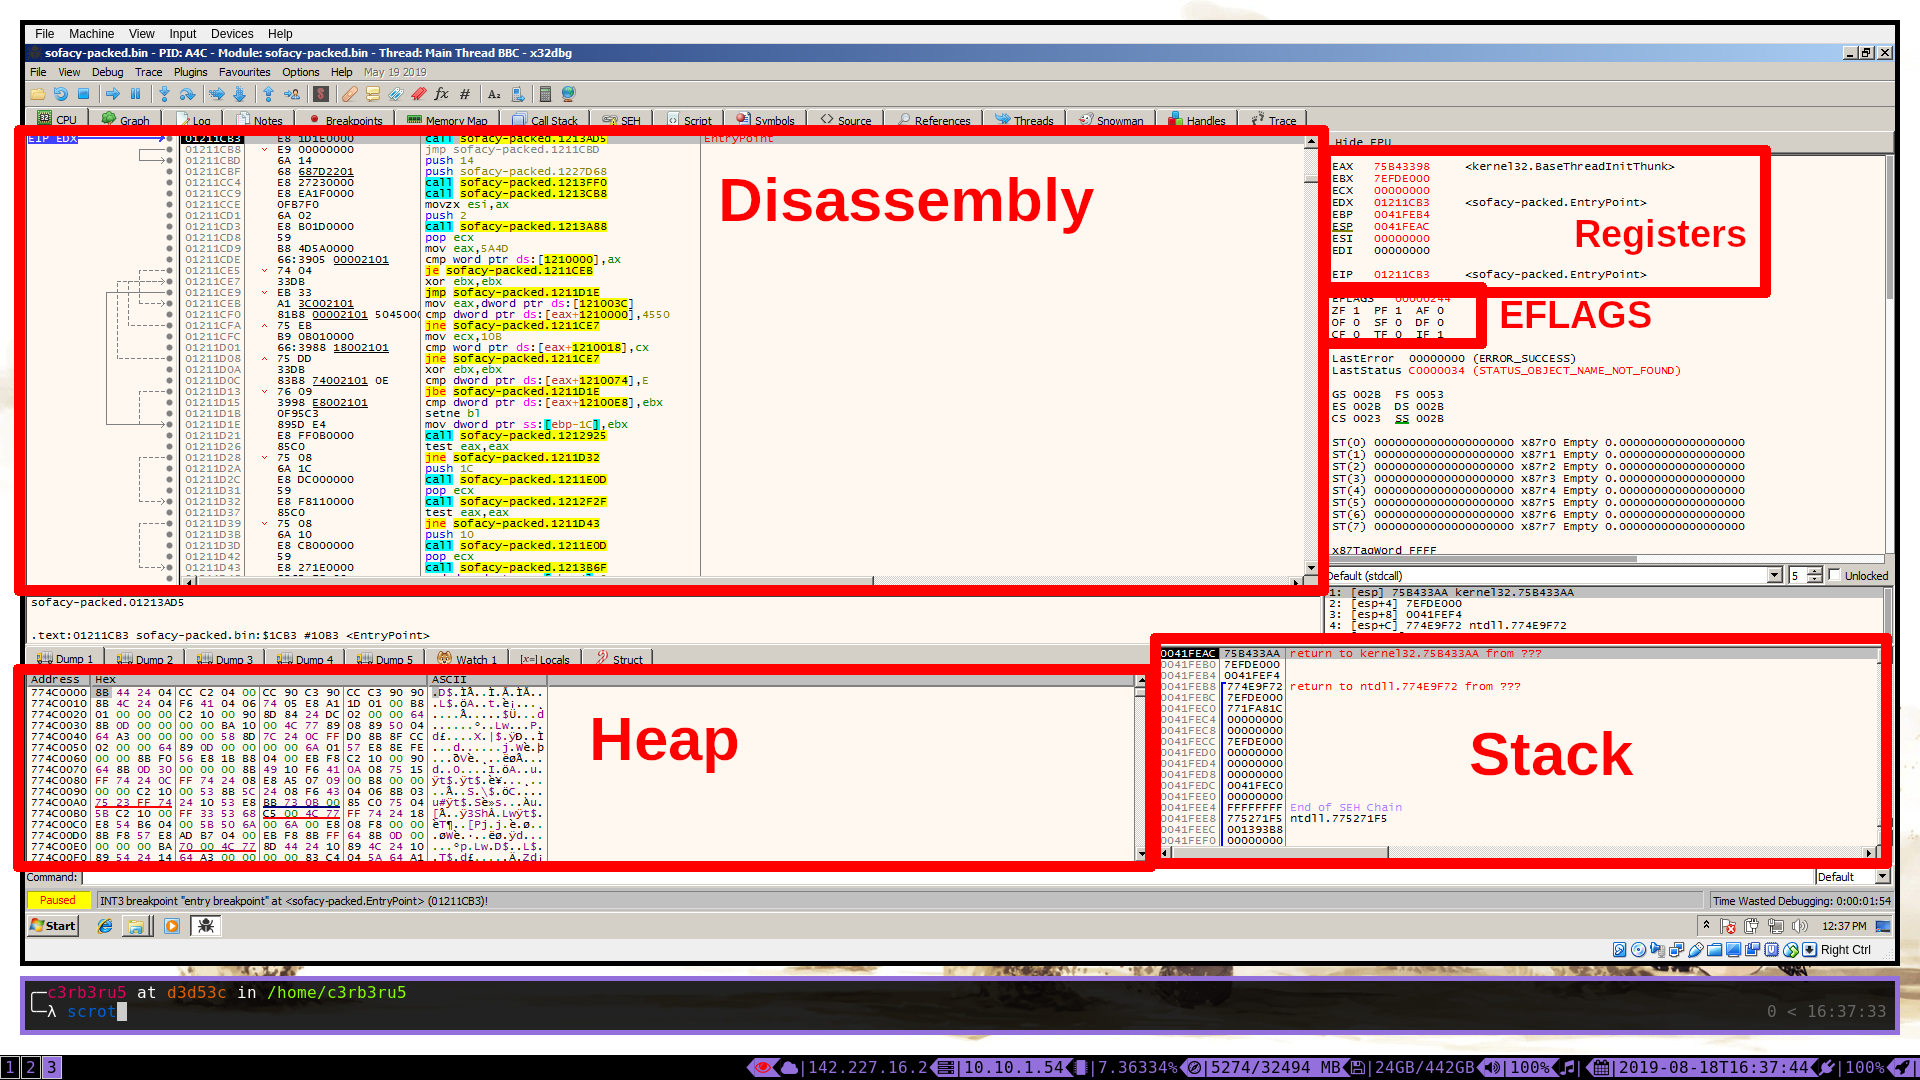
\includegraphics[scale=0.75]{x64dbg-overview}
  \end{center}
\end{frame}

\begin{frame}
  \frametitle{x64dbg}
  \framesubtitle{tools\_of\_the\_trade: 0x03}
  \begin{center}
    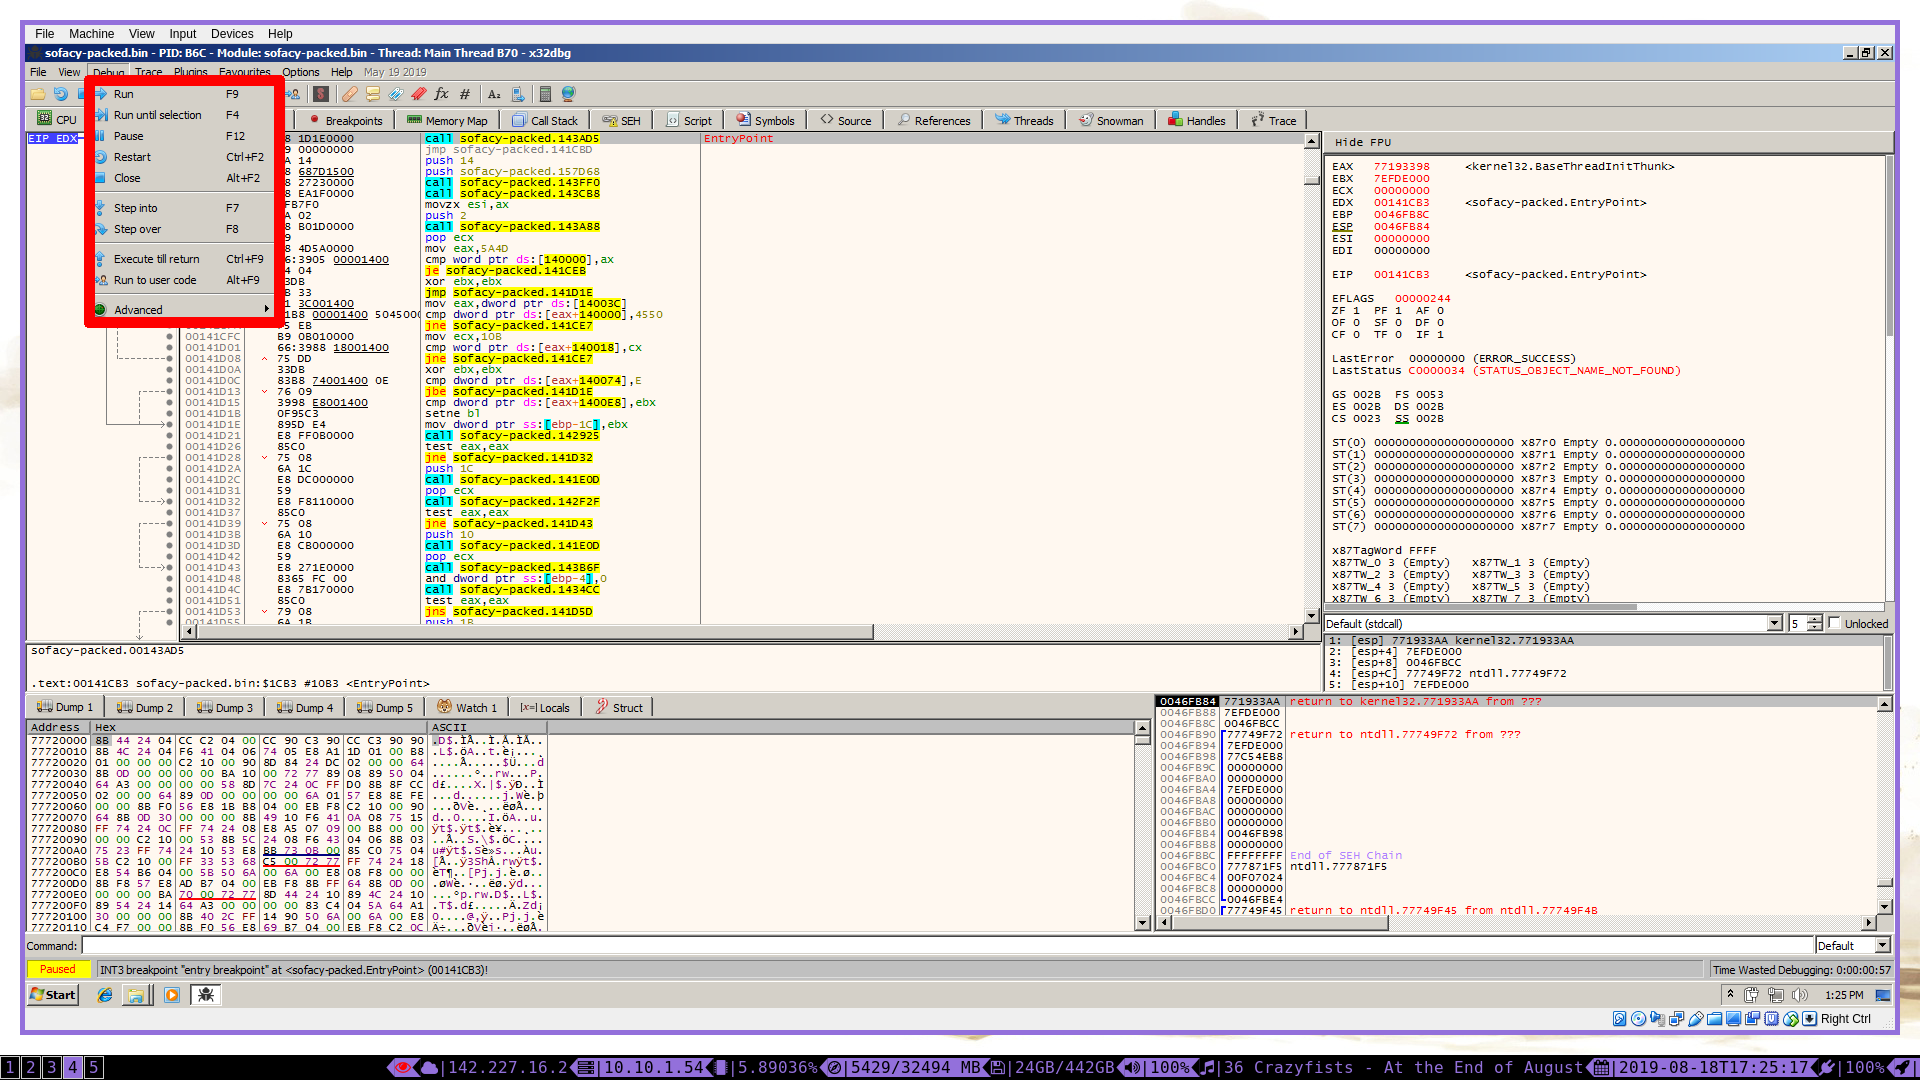
\includegraphics[scale=0.75]{x64dbg-navigation}
  \end{center}
\end{frame}

\begin{frame}
  \frametitle{x64dbg}
  \framesubtitle{tools\_of\_the\_trade: 0x04}
  \begin{center}
    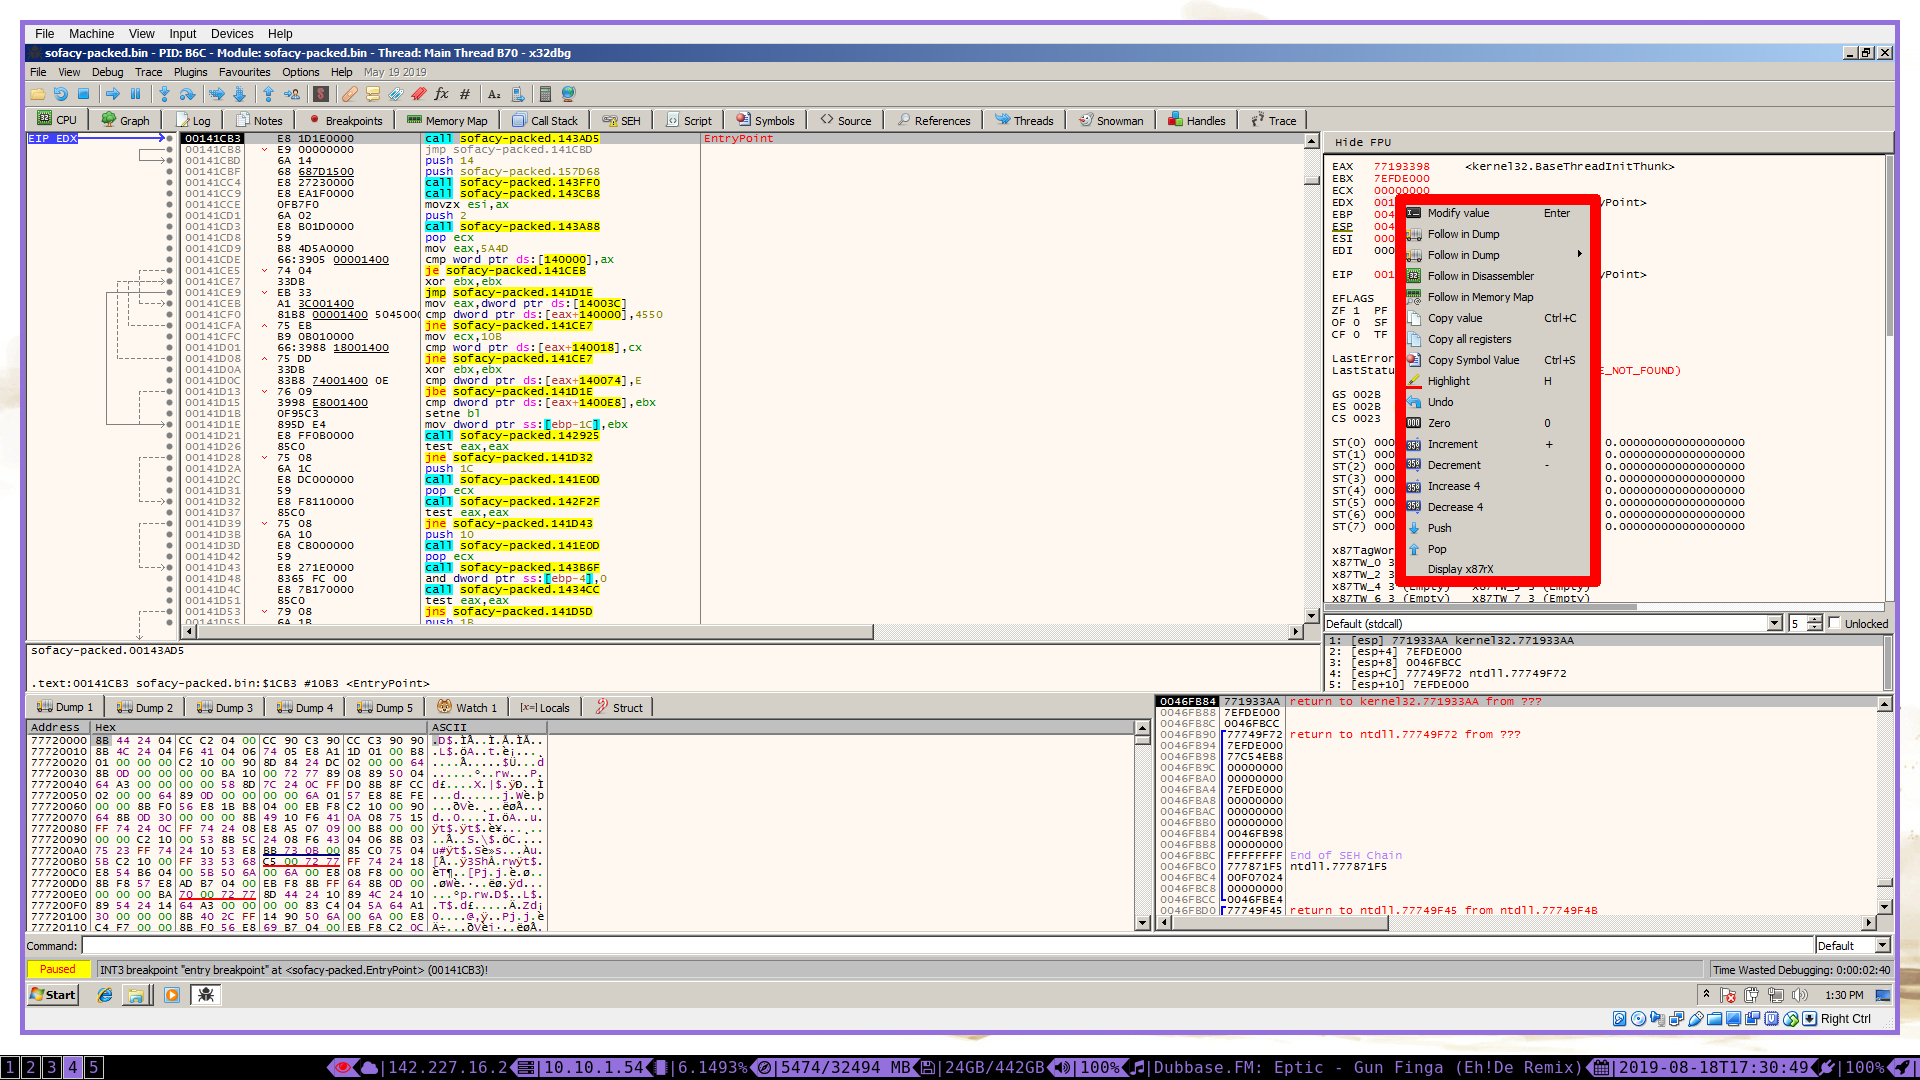
\includegraphics[scale=0.75]{x64dbg-context-menu}
  \end{center}
\end{frame}

\begin{frame}
  \frametitle{Cutter}
  \framesubtitle{tools\_of\_the\_trade: 0x05}
  \begin{columns}
    \begin{column}{.3\textwidth}
      \begin{itemize}
      \item{Markup Reverse Engineered Code}
      \item{Control Flow Navigation}
      \item{Pseudo Code}
      \end{itemize}
    \end{column}
    \hfill
    \begin{column}{.7\textwidth}
      \begin{center}
        
\includegraphics[scale=0.4]{ida-pro-meme}
      \end{center}
    \end{column}
  \end{columns}
\end{frame}

\begin{frame}
  \frametitle{Cutter}
  \framesubtitle{tools\_of\_the\_trade: 0x06}
  \begin{center}
    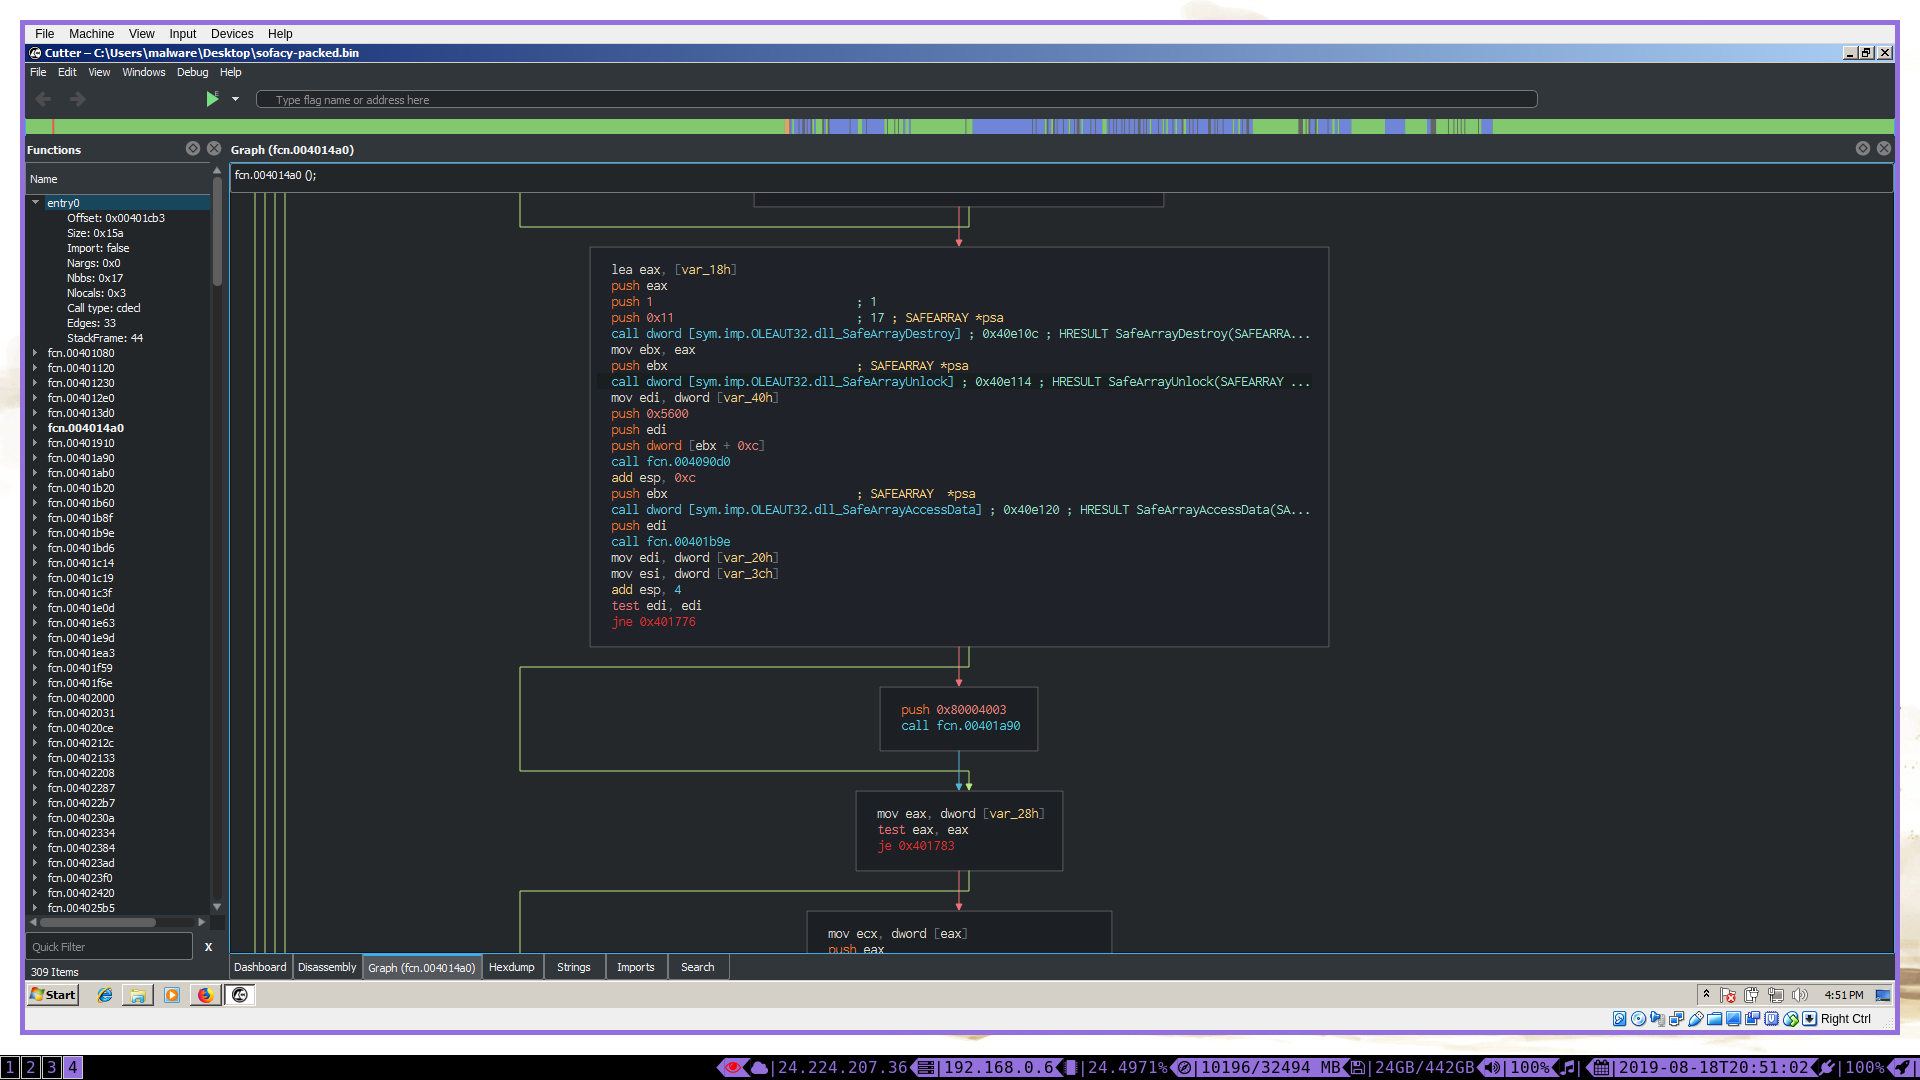
\includegraphics[scale=0.18]{cutter-graph}
  \end{center}
\end{frame}

\begin{frame}
  \frametitle{Cutter}
  \framesubtitle{tools\_of\_the\_trade: 0x07}
  \begin{center}
    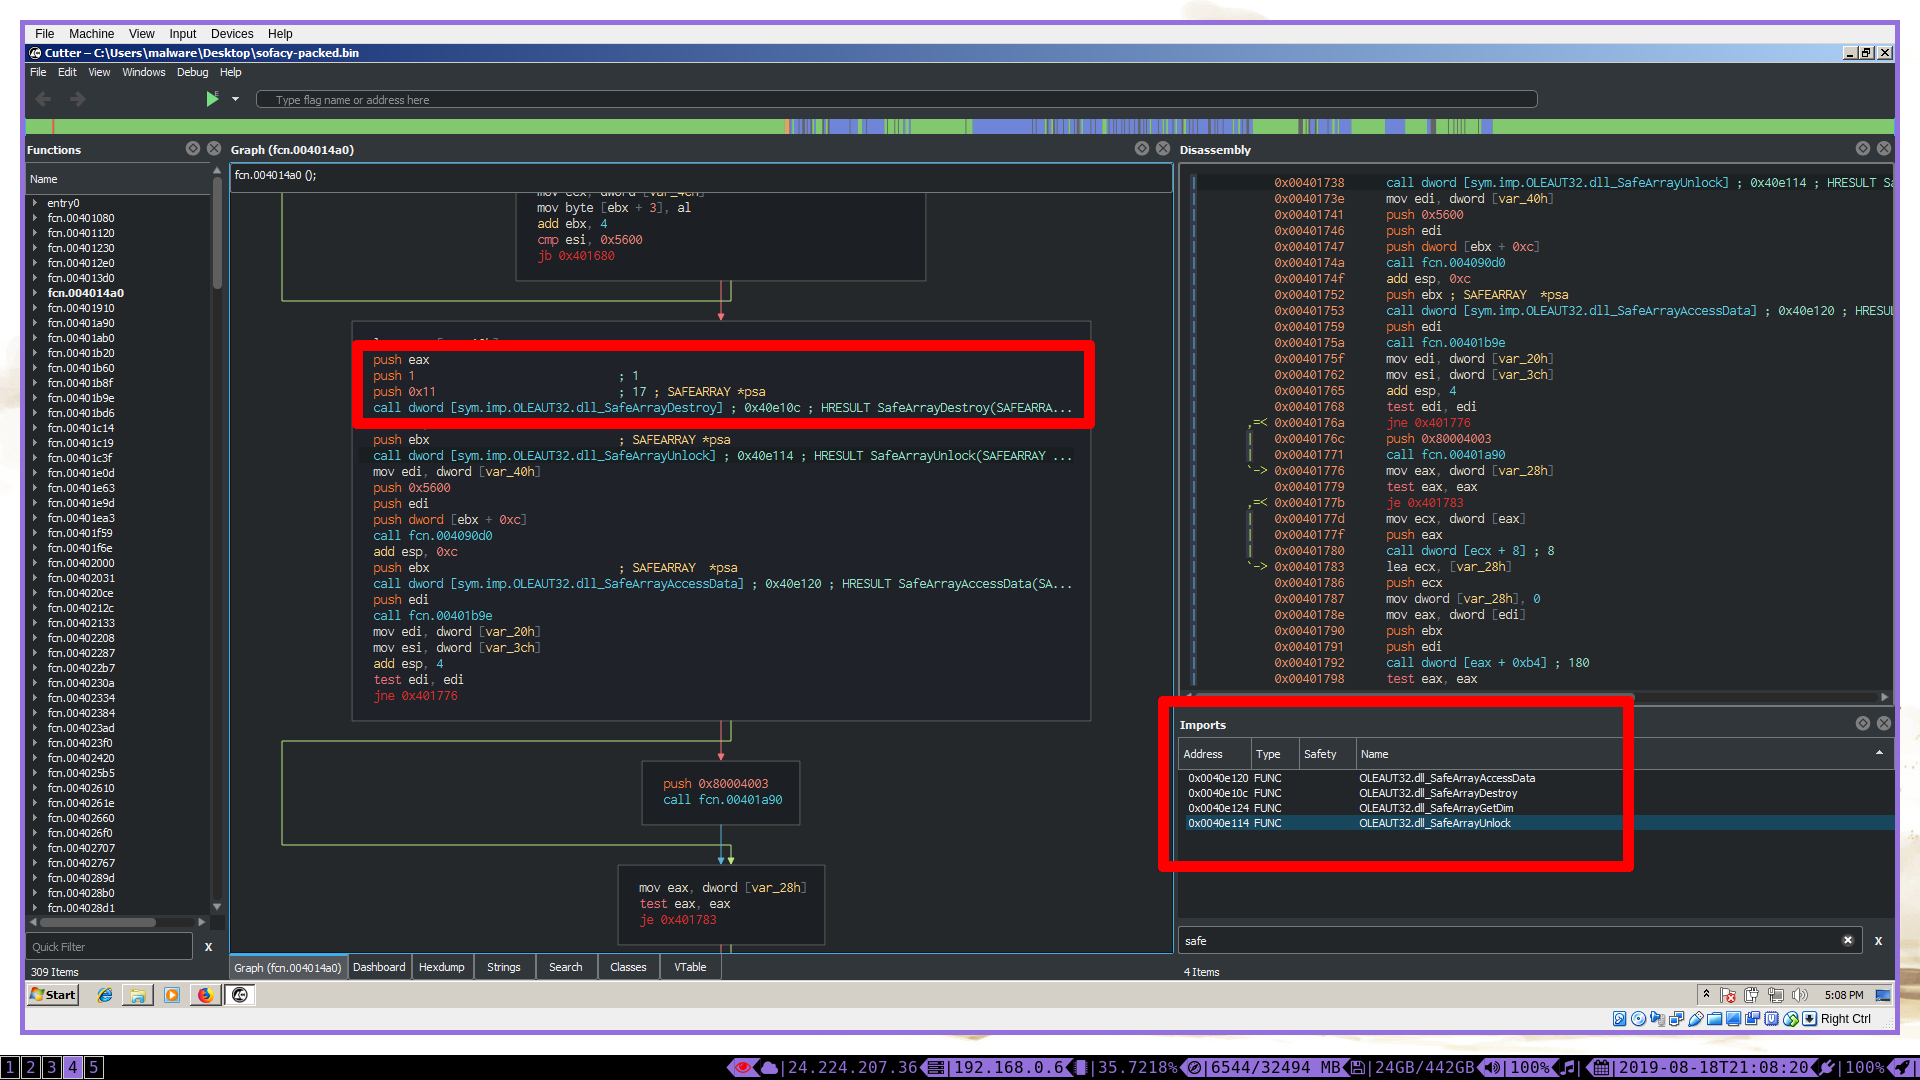
\includegraphics[scale=0.75]{cutter-navigation}
  \end{center}
\end{frame}

\begin{frame}
  \frametitle{Radare2}
  \framesubtitle{tools\_of\_the\_trade: 0x08}
  \begin{center}
    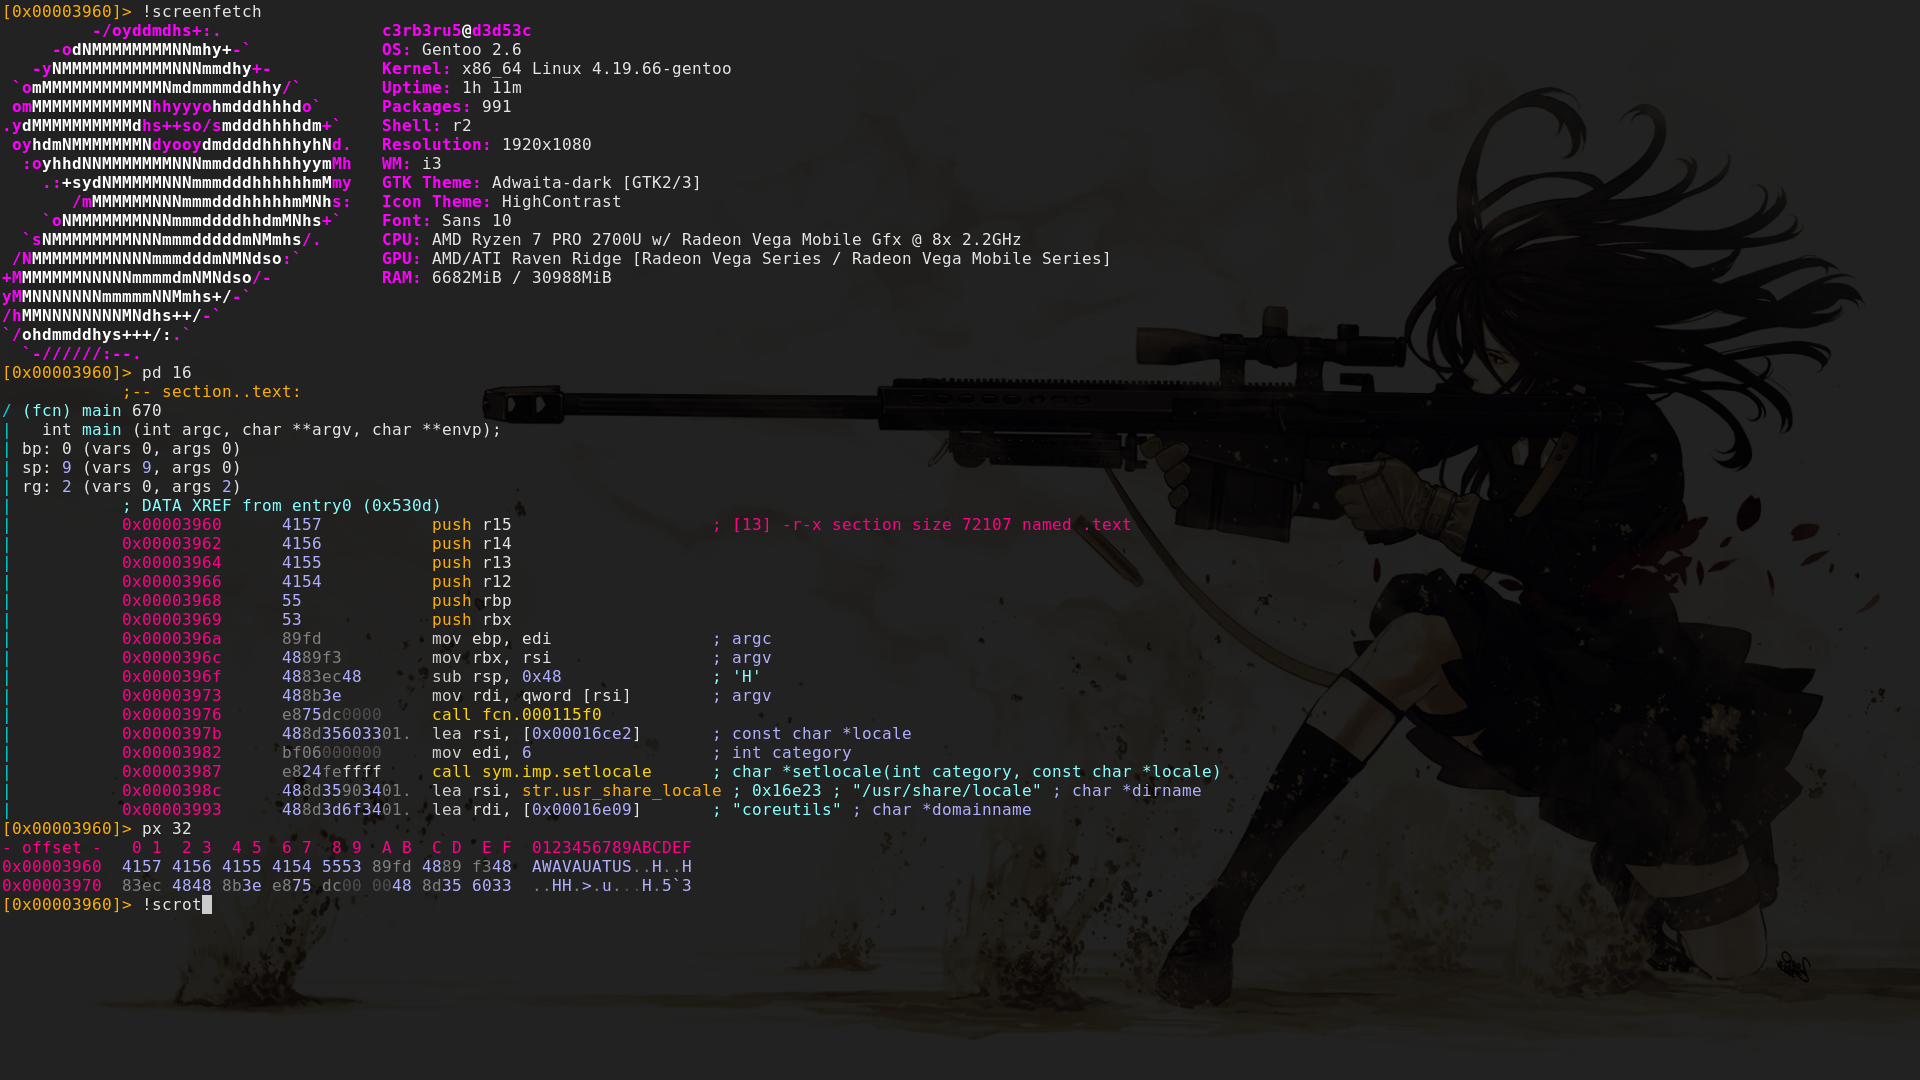
\includegraphics[scale=0.18]{radare2}
  \end{center}
\end{frame}

\begin{frame}
  \frametitle{Detect it Easy}
  \framesubtitle{tools\_of\_the\_trade: 0x09}
  \begin{columns}
    \begin{column}{.2\textwidth}
      \begin{itemize}
      \item{Type}
      \item{Packer}
      \item{Linker}
      \item{Entropy}
      \end{itemize}
    \end{column}
    \hfill
    \begin{column}{.8\textwidth}
      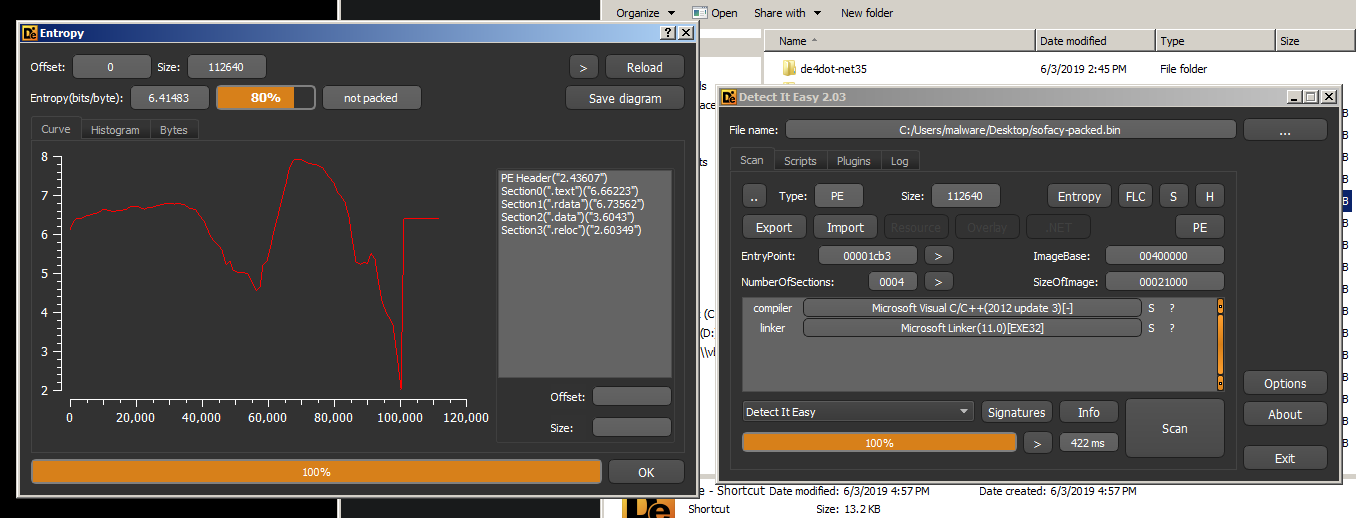
\includegraphics[scale=.98]{detect-it-easy}
    \end{column}
  \end{columns}
\end{frame}

\begin{frame}
  \frametitle{HxD}
  \framesubtitle{tools\_of\_the\_trade: 0x0a}
  \begin{columns}
    \begin{column}{.3\textwidth}
      \begin{itemize}
      \item{Modify Dumps}
      \item{Read Memory}
      \item{Determine File Type}
      \end{itemize}
    \end{column}
    \hfill
    \begin{column}{.7\textwidth}
      \begin{center}
        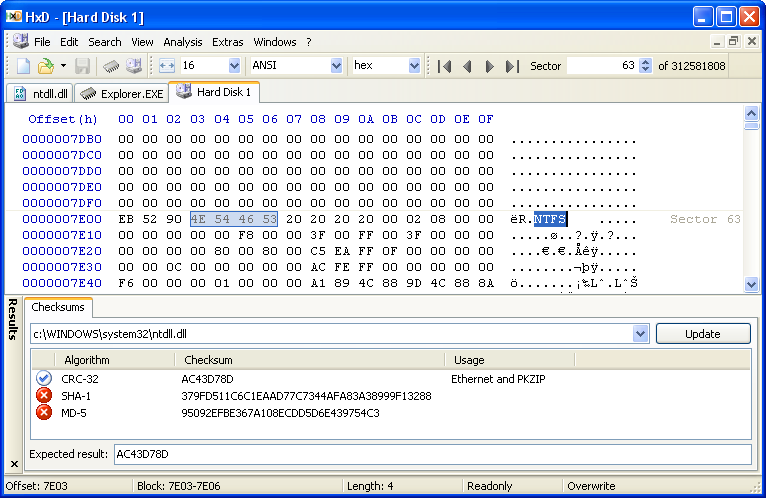
\includegraphics[scale=0.35]{hxd}
      \end{center}
    \end{column}
  \end{columns}
\end{frame}

\begin{frame}
  \frametitle{DnSpy}
  \framesubtitle{tools\_of\_the\_trade: 0x0b}
  \begin{columns}
    \begin{column}{.3\textwidth}
      \begin{itemize}
        \item{Code View}
        \item{Debugging}
        \item{Unpacking}
      \end{itemize}
    \end{column}
    \hfill
    \begin{column}{.7\textwidth}
      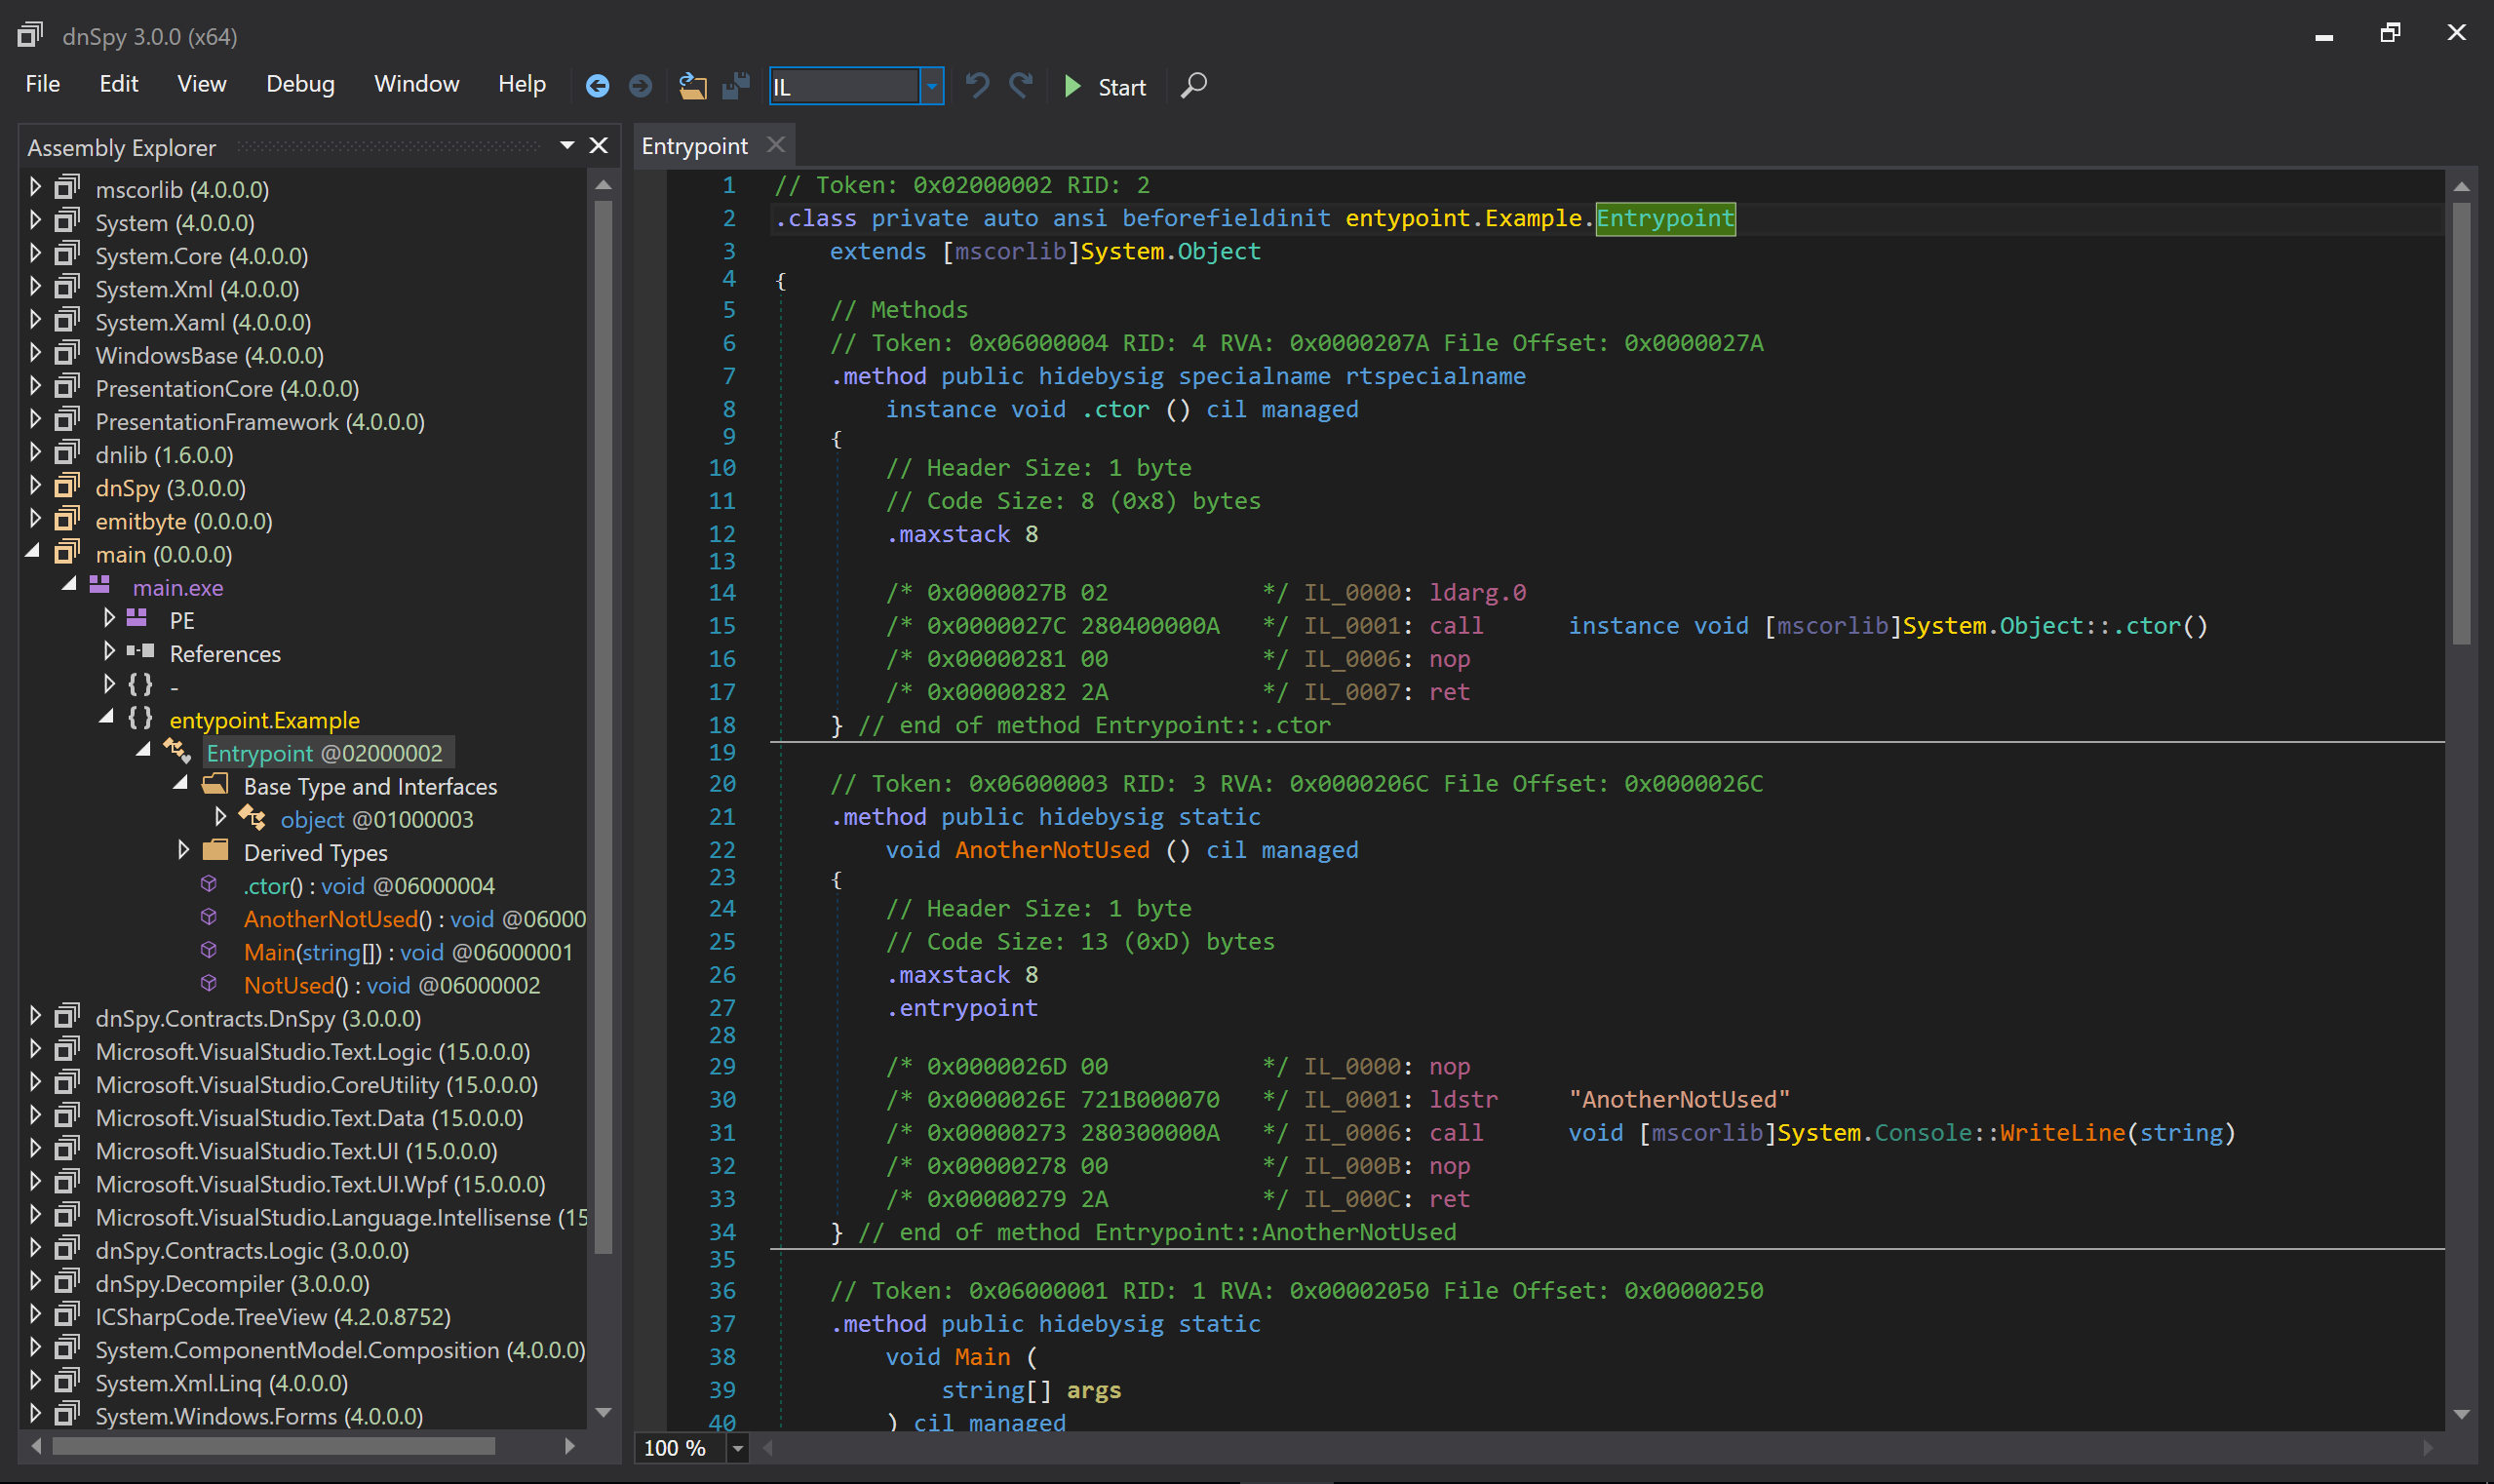
\includegraphics[scale=0.22]{dnspy}
    \end{column}
  \end{columns}
\end{frame}

\begin{frame}
  \frametitle{Useful Linux Commads}
  \framesubtitle{tools\_of\_the\_trade: 0x0c}
  \begin{center}
    \begin{tcolorbox}[title=terminal,colback=black]
      \begin{minipage}{0.8\textwidth}
        \textbf{\textcolor{green}{malware@work \textcolor{blue}{\~ \$}}}
        \textcolor{white}{ file sample.bin}
        \newline
        \textcolor{white}{ sample.bin: PE32 executable (GUI) Intel 80386, for MS Windows}
        \newline
        \textbf{\textcolor{green}{malware@work \textcolor{blue}{\~ \$}}}
        \textcolor{white}{ exiftool sample.bin $>$ metadata.log}
        \newline
        \textbf{\textcolor{green}{malware@work \textcolor{blue}{\~ \$}}} \textcolor{white}{ hexdump -C -n 128 sample.bin $|$ less}
        \newline
        \textbf{\textcolor{green}{malware@work \textcolor{blue}{\~ \$}}}
        \textcolor{white}{ VBoxManage list vms}
        \newline
        \textcolor{white}{"win10" \{53014b4f-4c94-49b0-9036-818b84a192c9\}\newline"win7" \{942cde2e-6a84-4edc-b98a-d7326b4662ee\}}
        \newline
        \textbf{\textcolor{green}{malware@work \textcolor{blue}{\~ \$}}}
        \textcolor{white}{ VBoxManage startvm win7}
        \newline
        \textbf{\textcolor{green}{malware@work \textcolor{blue}{\~ \$}}}
      \end{minipage}
    \end{tcolorbox}
  \end{center}
\end{frame}

\begin{frame}
  \frametitle{Injection Techniques}
  \begin{center}
    
\includegraphics[scale=.275]{injection-meme}
  \end{center}
\end{frame}

\begin{frame}
  \frametitle{DLL Injection}
  \framesubtitle{injection\_techniques: 0x00}
  \begin{columns}
    \begin{column}{.3\textwidth}
      \begin{itemize}
      \item{Get Handle to Target Process}
      \item{Allocate Memory}
      \item{Write Memory}
      \item{Execute by use of Remote Thread} 
      \end{itemize}
    \end{column}
    \hfill
    \begin{column}{.7\textwidth}
      \begin{center}
        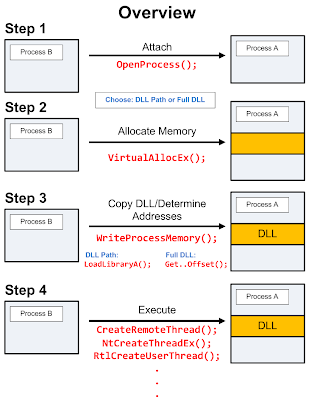
\includegraphics[scale=0.5]{dll-injection}
      \end{center}
    \end{column}
  \end{columns}
\end{frame}

\begin{frame}
  \frametitle{PE (Portable Executable) Injection}
  \framesubtitle{injection\_techniques: 0x01}
  \begin{columns}
    \begin{column}{.5\textwidth}
      \begin{itemize}
      \item{Obtain Handle to Target Process}
      \item{Inject Image to Target Process}
      \item{Modify Base Address}
      \item{Modify Relocation Table}
      \item{Execute your Payload}
      \end{itemize}
    \end{column}
    \hfill
    \begin{column}{.5\textwidth}
      \begin{center}
        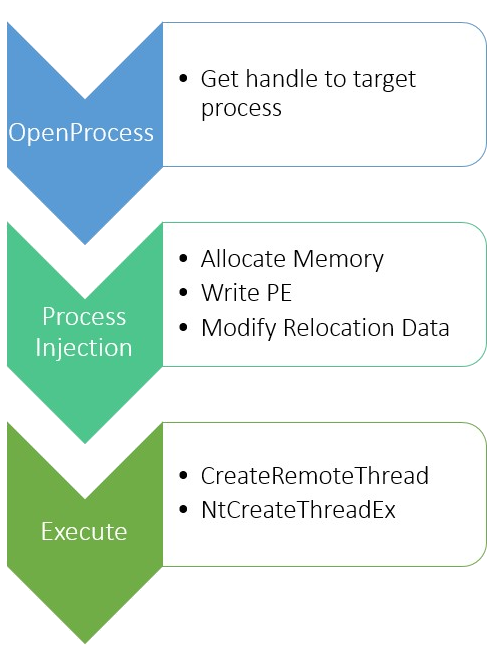
\includegraphics[scale=0.5]{pe-injection}
      \end{center}
    \end{column}
  \end{columns}
\end{frame}

\begin{frame}
  \frametitle{Process Hollowing}
  \framesubtitle{injection\_techniques: 0x02}
  \begin{columns}
    \begin{column}{.5\textwidth}
      \begin{itemize}
      \item{Create Suspended Process}
      \item{Hollow Process with NtUnmapViewOfSection}
      \item{Allocate Memory in Process}
      \item{Write Memory to Process}
      \item{Resume Thread / Process}
      \end{itemize}
    \end{column}
    \hfill
    \begin{column}{.5\textwidth}
      \begin{center}
        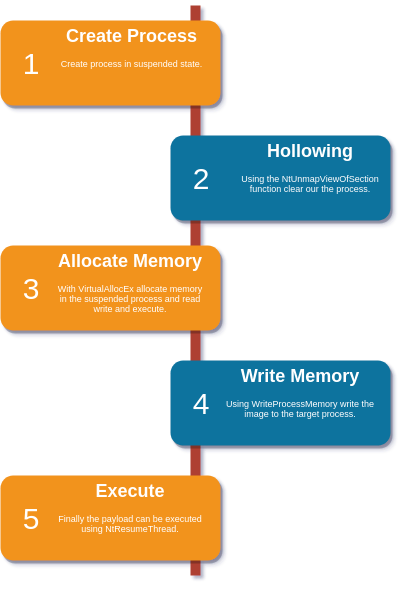
\includegraphics[scale=0.35]{process-hollowing}
      \end{center}
    \end{column}
  \end{columns}
\end{frame}

\begin{frame}
  \frametitle{Atom Bombing}
  \framesubtitle{injection\_techniques: 0x04}
  \begin{center}
    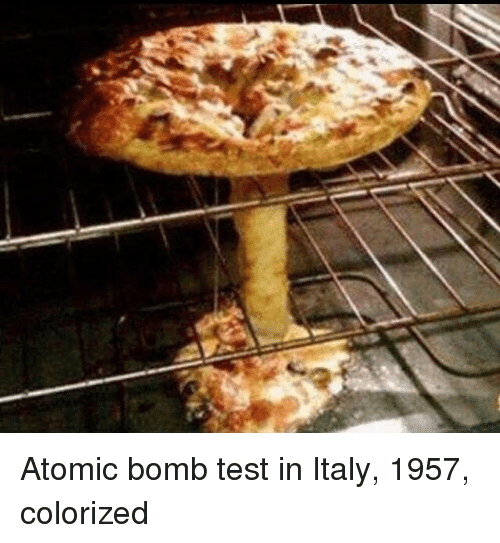
\includegraphics[scale=0.36]{atom-bomb-meme}
  \end{center}
\end{frame}

\begin{frame}
  \frametitle{Atom Bombing}
  \framesubtitle{injection\_techniques: 0x05}
  \begin{columns}
    \begin{column}{.4\textwidth}
      \begin{itemize}
        \item{Open Target Process}
        \item{Get Handle to Alertable Thread}
        \item{Find Code Cave}
        \item{Shellcode to Call ZwAllocateVirtualMemory and memcpy}
        \item{Call GlobalAddAtom}
        \item {Suspend Target Thread}
        \item{NtQueueApcThread}
        \item{Resume Target Thread}
      \end{itemize}
    \end{column}
    \hfill
    \begin{column}{.6\textwidth}
      \begin{center}
        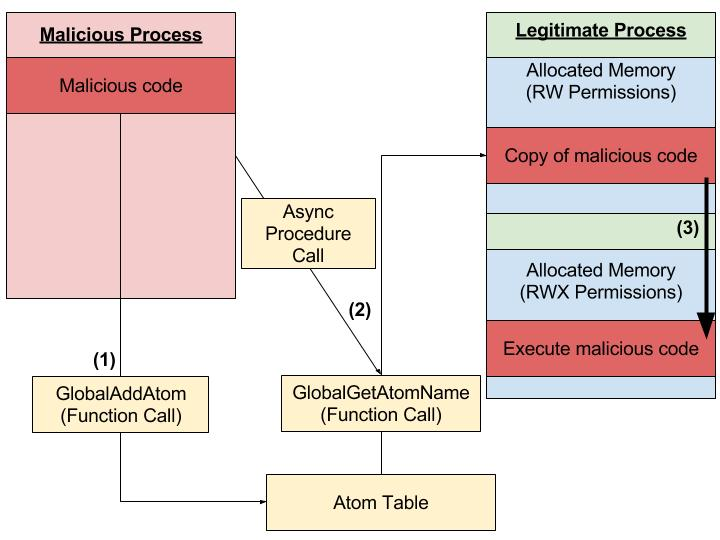
\includegraphics[scale=0.30]{atom-bombing}
      \end{center}
    \end{column}
  \end{columns}
  % An atom table is a system-defined table that stores strings and corresponding identifiers. An application places a string in an atom table and receives a 16-bit integer, called an atom, that can be used to access the string. A string that has been placed in an atom table is called an atom name.
\end{frame}

\begin{frame}
  \frametitle{Workshop}
  \begin{columns}
    \begin{column}{.3\textwidth}
      \begin{itemize}
      \item{NJRat}
      \item{Sofacy}
      \item{KPot}
      \item{Stuxnet}
      \end{itemize}
    \end{column}
    \hfill
    \begin{column}{.7\textwidth}
      \begin{center}
        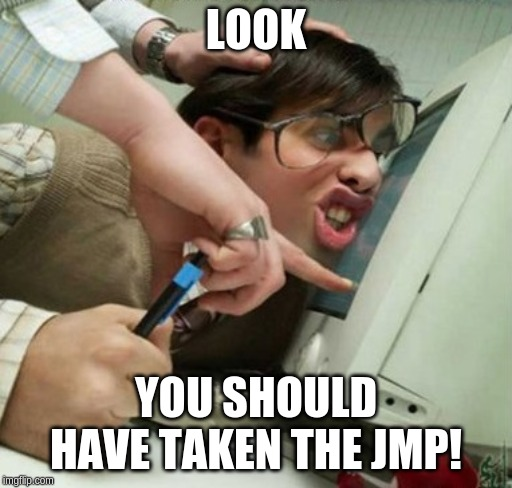
\includegraphics[scale=0.4]{jmp-meme}
      \end{center}
    \end{column}
  \end{columns}
\end{frame}

\begin{frame}
  \frametitle{Unpacking NJRat}
  \framesubtitle{solutions: 0x00}
  \begin{columns}
    \begin{column}{.5\textwidth}
      \begin{itemize}
      \item{Determine the File Type}
      \item{Because this is .NET we may wish to use DnSpy}
      \item{Let's see if it's packed now}
      \end{itemize}
    \end{column}
    \hfill
    \begin{column}{.5\textwidth}
      \begin{center}
        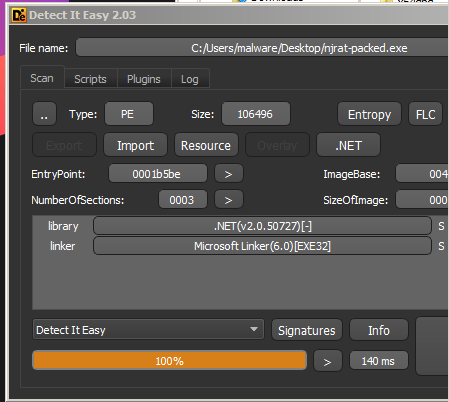
\includegraphics[scale=1.5]{njrat-detect-it-easy}
      \end{center}
    \end{column}
  \end{columns}
\end{frame}

\begin{frame}
  \frametitle{Unpacking NJRat}
  \framesubtitle{solutions: 0x01}
  \begin{columns}
    \begin{column}{.5\textwidth}
      \begin{itemize}
      \item{Low Entropy?}
      \item{Look at the beginning}
      \item{We should now look into the code using DnSpy}
      \end{itemize}
    \end{column}
    \hfill
    \begin{column}{.5\textwidth}
      \begin{center}
        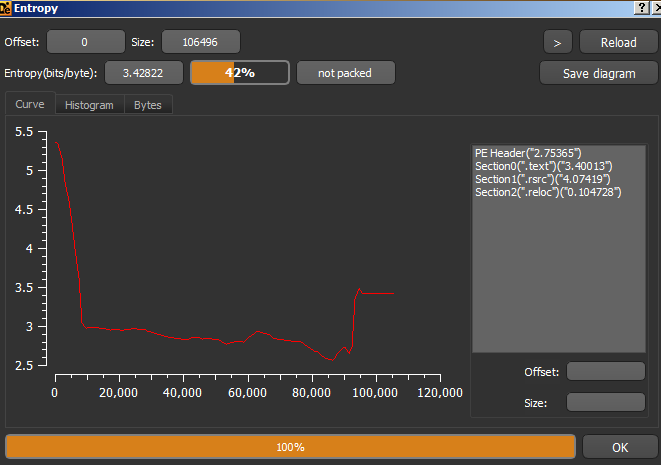
\includegraphics[scale=1.2]{njrat-detect-it-easy-entropy}
      \end{center}
    \end{column}
  \end{columns}
\end{frame}

\begin{frame}
  \frametitle{Unpacking NJRat}
  \framesubtitle{solutions:0x02}
  \begin{columns}
    \begin{column}{.3\textwidth}
      \begin{itemize}
      \item{Assembly.Load}
      \item{Set Breakpoint on this function}
      \item{Start Debugging}
      \end{itemize}
    \end{column}
    \hfill
    \begin{column}{.7\textwidth}
      \begin{center}
        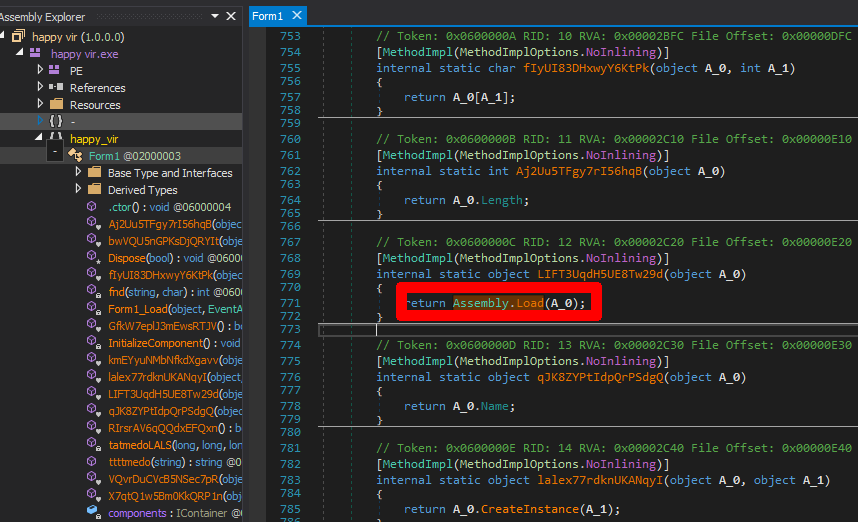
\includegraphics[scale=1.25]{njrat-assembly-load}
      \end{center}
    \end{column}
  \end{columns}
\end{frame}

\begin{frame}
  \frametitle{Unpacking NJRat}
  \framesubtitle{solutions: 0x03}
  \begin{columns}
    \begin{column}{.3\textwidth}
      \begin{itemize}
      \item{Breakpoint on Assembly.Load}
      \item{Save the Raw Array to Disk}
      \end{itemize}
    \end{column}
    \hfill
    \begin{column}{.7\textwidth}
      \begin{center}
        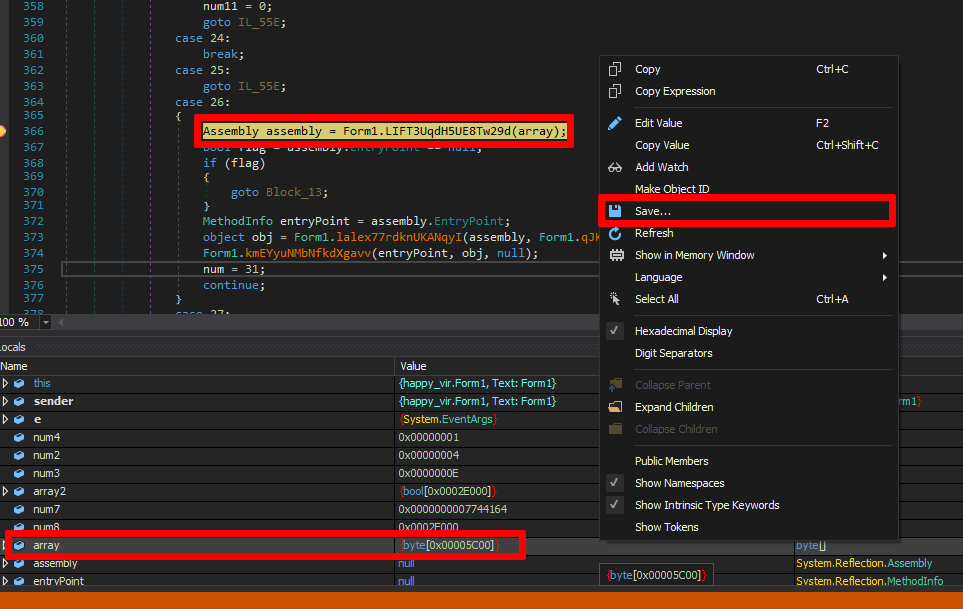
\includegraphics[scale=1.2]{njrat-dump-assembly}
      \end{center}
    \end{column}
  \end{columns}
\end{frame}

\begin{frame}
  \frametitle{Unpacking NJRat}
  \framesubtitle{solutions: 0x04}
  \begin{columns}
    \begin{column}{.3\textwidth}
      \begin{itemize}
      \item{MZ at the beginning}
      \item{Appears to be the Payload}
      \item{Let's see what kind of file it is}
      \end{itemize}
    \end{column}
    \hfill
    \begin{column}{.7\textwidth}
      \begin{center}
        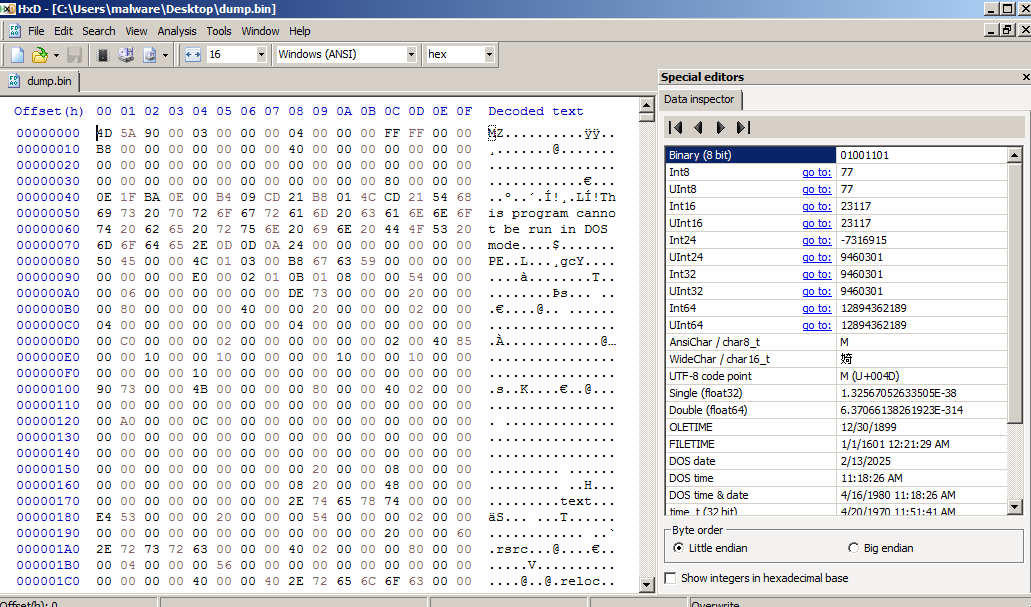
\includegraphics[scale=1]{njrat-unpacked-hex}
      \end{center}
    \end{column}
  \end{columns}
\end{frame}


\begin{frame}
  \frametitle{Unpacking NJRat}
  \framesubtitle{solutions: 0x05}
  \begin{columns}
    \begin{column}{.4\textwidth}
      \begin{itemize}
      \item{Looks like .NET Again}
      \item{Let's look at DnSpy}
      \end{itemize}
    \end{column}
    \hfill
    \begin{column}{.6\textwidth}
      \begin{center}
        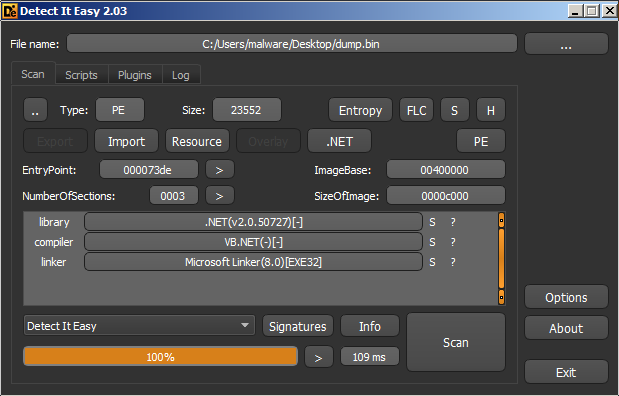
\includegraphics[scale=1.2]{njrat-unpacked-detect-it-easy}
      \end{center}
    \end{column}
  \end{columns}
\end{frame}

\begin{frame}
  \frametitle{Unpacking NJRat}
  \framesubtitle{solutions: 0x06}
  \begin{columns}
    \begin{column}{.25\textwidth}
      \begin{itemize}
      \item{Keylogger Code}
      \item{CnC Traffic Code}
      \end{itemize}
    \end{column}
    \hfill
    \begin{column}{.75\textwidth}
      \begin{center}
        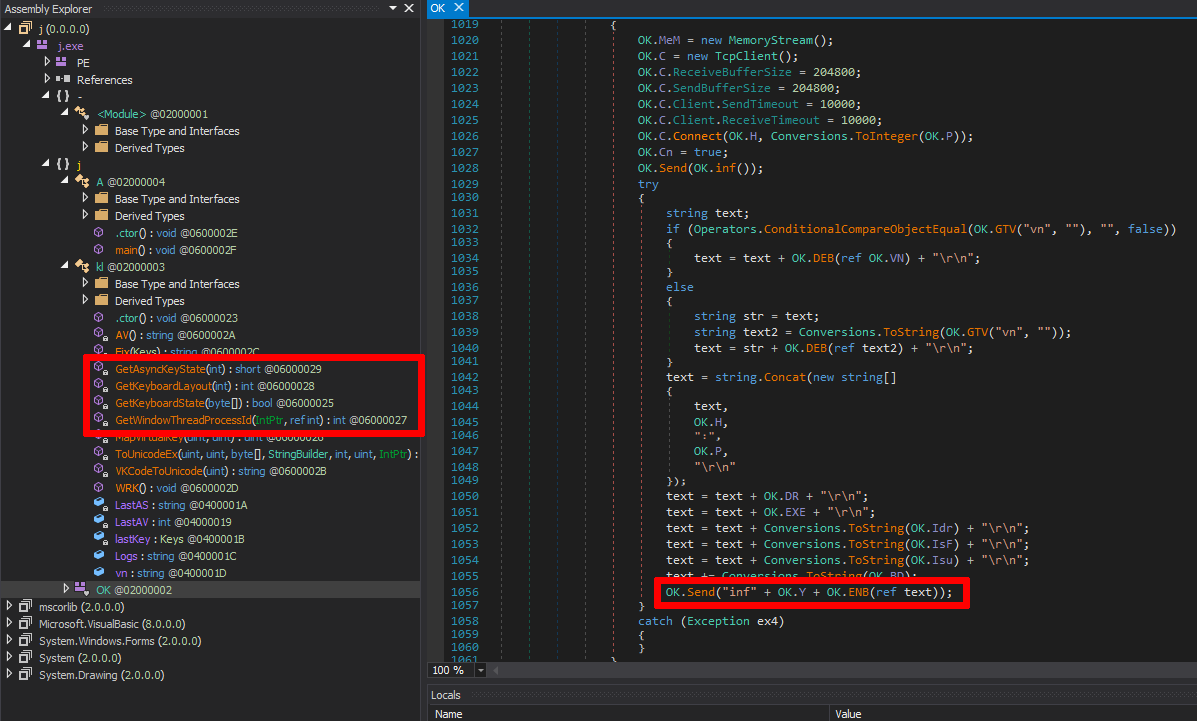
\includegraphics[scale=1]{njrat-unpacked-code-0}
      \end{center}
    \end{column}
  \end{columns}
\end{frame}

\begin{frame}
  \frametitle{Unpacking NJRat}
  \framesubtitle{solutions: 0x07}
  \begin{columns}
    \begin{column}{.3\textwidth}
      \begin{itemize}
      \item{CnC Server IP Address}
      \item{CnC Keyword}
      \end{itemize}
    \end{column}
    \hfill
    \begin{column}{.7\textwidth}
      \begin{center}
        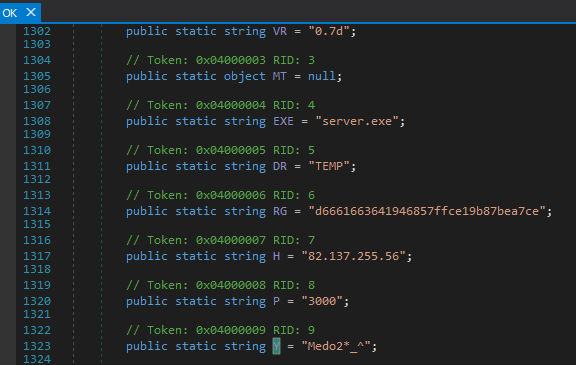
\includegraphics[scale=1.75]{njrat-unpacked-code-1}
      \end{center}
    \end{column}
  \end{columns}
\end{frame}

\begin{frame}
  \frametitle{Unpacking Sofacy / FancyBear}
  \framesubtitle{solutions: 0x09}
  \begin{center}
    
\includegraphics[scale=0.5]{fancy-bear-logo}
  \end{center}
\end{frame}

\begin{frame}
  \frametitle{Unpacking Sofacy / FancyBear}
  \framesubtitle{solutions: 0x0a}
  \begin{columns}
    \begin{column}{.3\textwidth}
      \begin{itemize}
      \item{C++}
      \item{No Packer Detected}
      \item{Let's look at entropy}
      \end{itemize}
    \end{column}
    \hfill
    \begin{column}{.7\textwidth}
      \begin{center}
        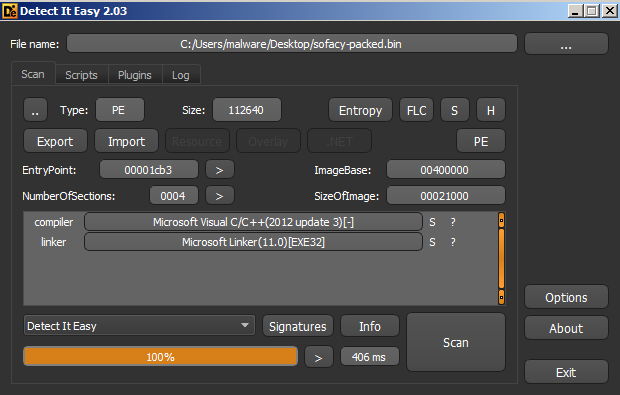
\includegraphics[scale=1.3]{sofacy-packed-detect-it-easy}
      \end{center}
    \end{column}
  \end{columns}
\end{frame}

\begin{frame}
  \frametitle{Unpacking Sofacy / FancyBear}
  \framesubtitle{solutions: 0x0b}
  \begin{columns}
    \begin{column}{.3\textwidth}
      \begin{itemize}
      \item{Not Packed?}
      \item{Let's look in x64dbg}
      \end{itemize}
    \end{column}
    \hfill
    \begin{column}{.7\textwidth}
      \begin{center}
        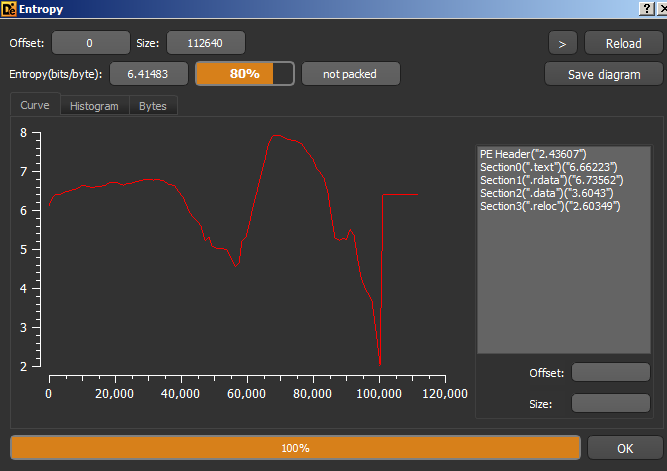
\includegraphics[scale=1.5]{sofacy-packed-detect-it-easy-entropy}
      \end{center}
    \end{column}
  \end{columns}
\end{frame}

\begin{frame}
  \frametitle{Unpacking Sofacy / FancyBear}
  \framesubtitle{solutions: 0x0c}
  \begin{center}
    \begin{figure}
      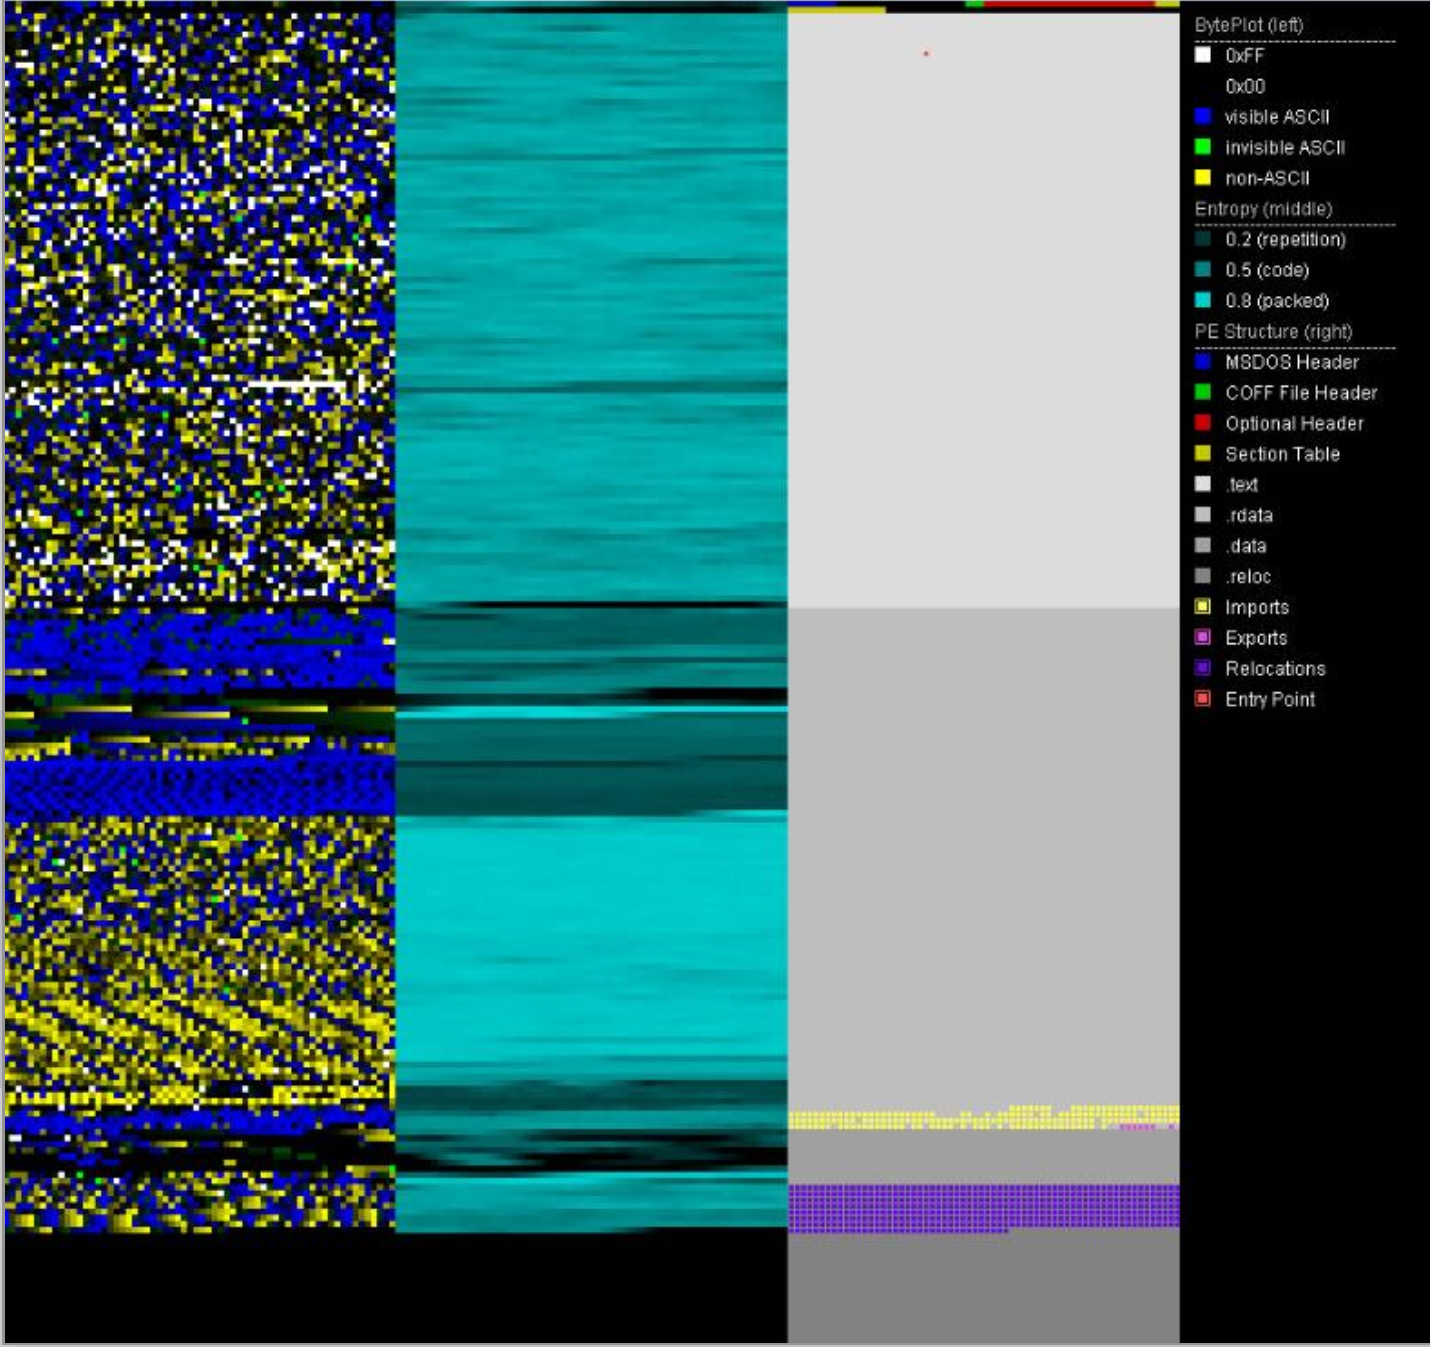
\includegraphics[scale=0.35]{fancy-bear-portexanalyzer}
      \caption{Sofacy / FancyBear - PortexAnalyzer}
    \end{figure}
  \end{center}
  NOTE: Some areas seem to have higher entropy than others!
\end{frame}

\begin{frame}
  \frametitle{Unpacking Sofacy / FancyBear}
  \framesubtitle{solutions: 0x0c}
  \begin{columns}
    \begin{column}{.3\textwidth}
      \begin{itemize}
      \item{Interesting Export}
      \end{itemize}
    \end{column}
    \hfill
    \begin{column}{.7\textwidth}
      \begin{center}
        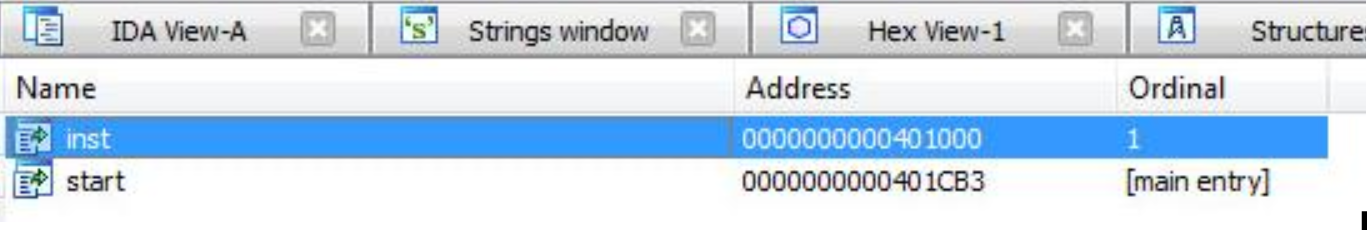
\includegraphics[scale=0.7]{fancy-bear-unpacking-0}
      \end{center}
    \end{column}
  \end{columns}
\end{frame}

\begin{frame}
  \frametitle{Unpacking Sofacy / FancyBear}
  \framesubtitle{solutions: 0x0d}
  \begin{columns}
    \begin{column}{.3\textwidth}
      \begin{itemize}
      \item{.NET Assembly Injection Method}
      \end{itemize}
    \end{column}
    \hfill
    \begin{column}{.7\textwidth}
      \begin{center}
        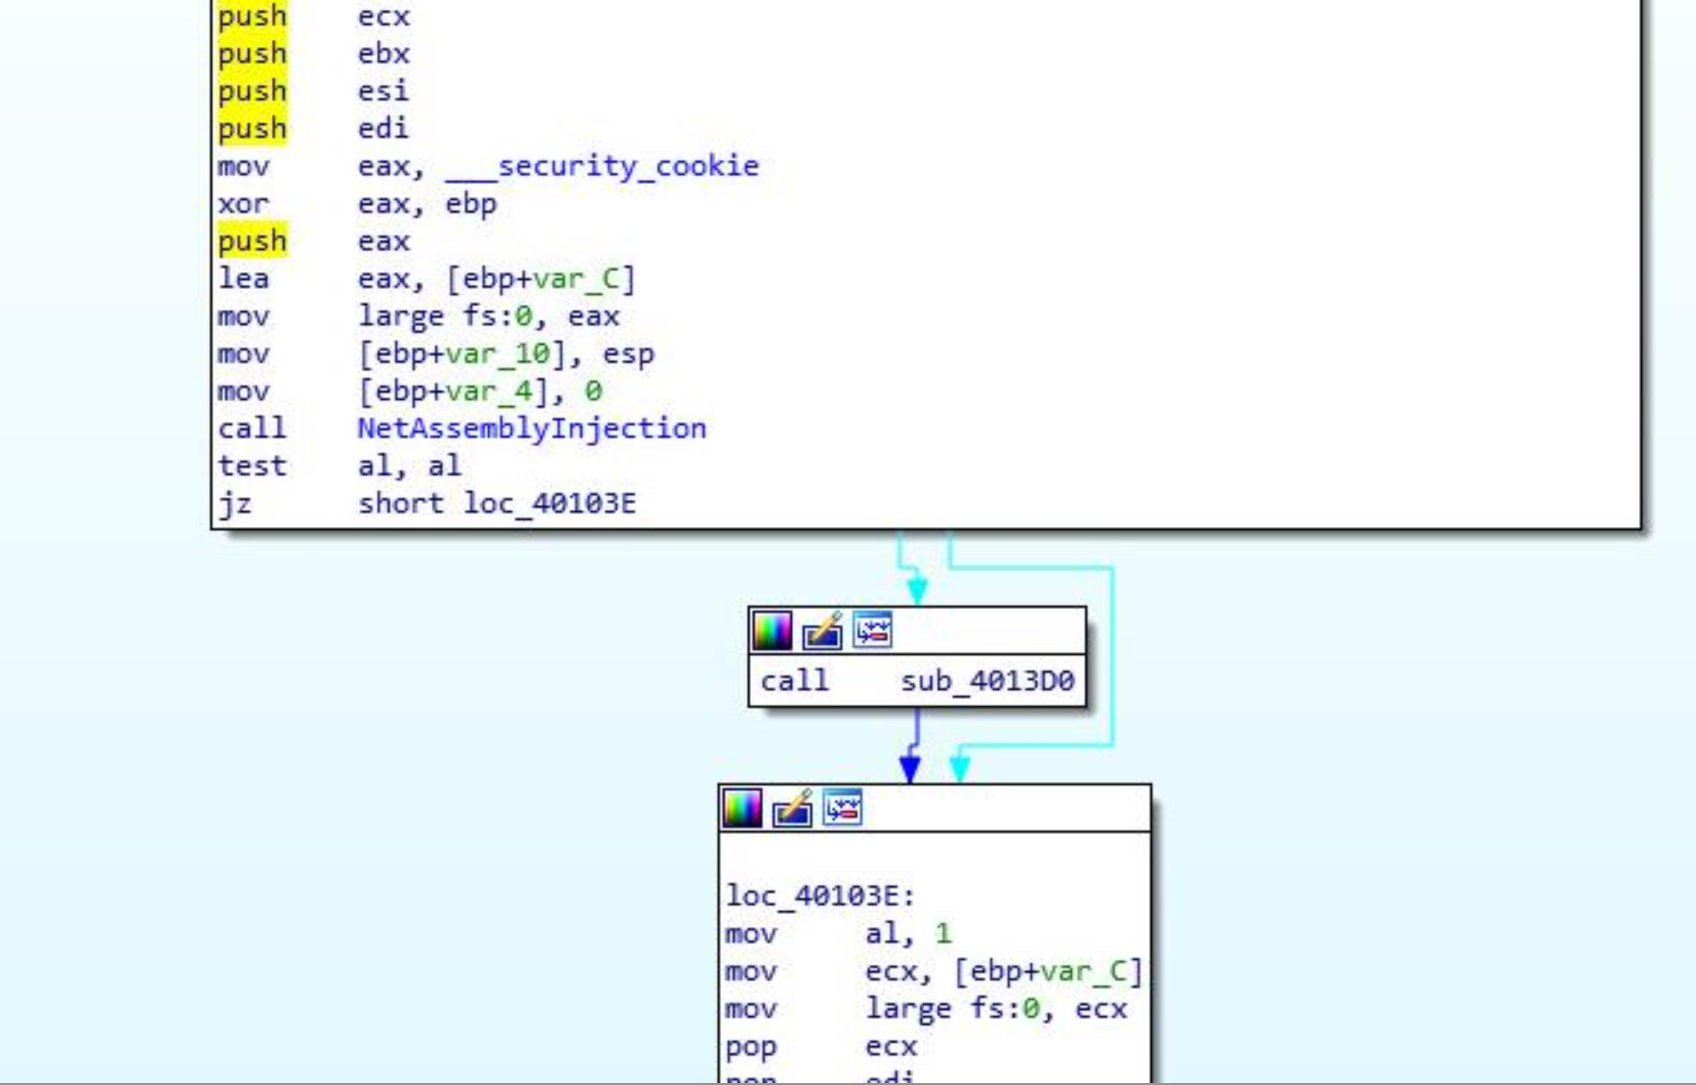
\includegraphics[scale=0.55]{fancy-bear-unpacking-1}
      \end{center}
    \end{column}
  \end{columns}
\end{frame}

\begin{frame}
  \frametitle{Unpacking Sofacy / FancyBear}
  \framesubtitle{solutions: 0x0e}
  \begin{columns}
    \begin{column}{.3\textwidth}
      \begin{itemize}
      \item{Create .NET Instance}
      \end{itemize}
    \end{column}
    \hfill
    \begin{column}{.7\textwidth}
      \begin{center}
        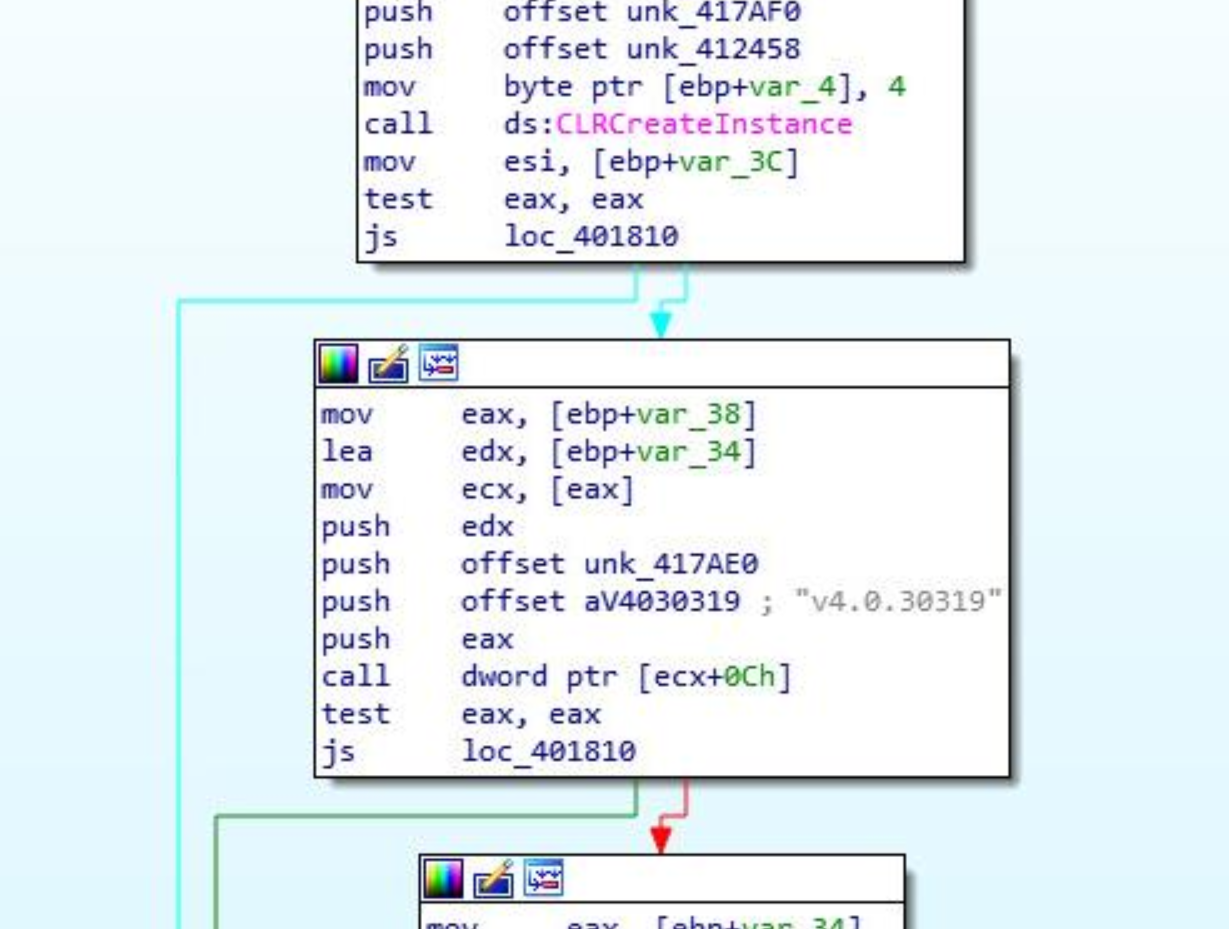
\includegraphics[scale=0.7]{fancy-bear-unpacking-2}
      \end{center}
    \end{column}
  \end{columns}
\end{frame}

\begin{frame}
  \frametitle{Unpacking Sofacy / FancyBear}
  \framesubtitle{solutions: 0x0e}
  \begin{columns}
    \begin{column}{.3\textwidth}
      \begin{itemize}
      \item{SafeArrayLock}
      \item{SafeArrayUnlock}
      \item{SafeArrayDestroy}
      \item{What is happening between these?}
      \end{itemize}
    \end{column}
    \hfill
    \begin{column}{.7\textwidth}
      \begin{center}
        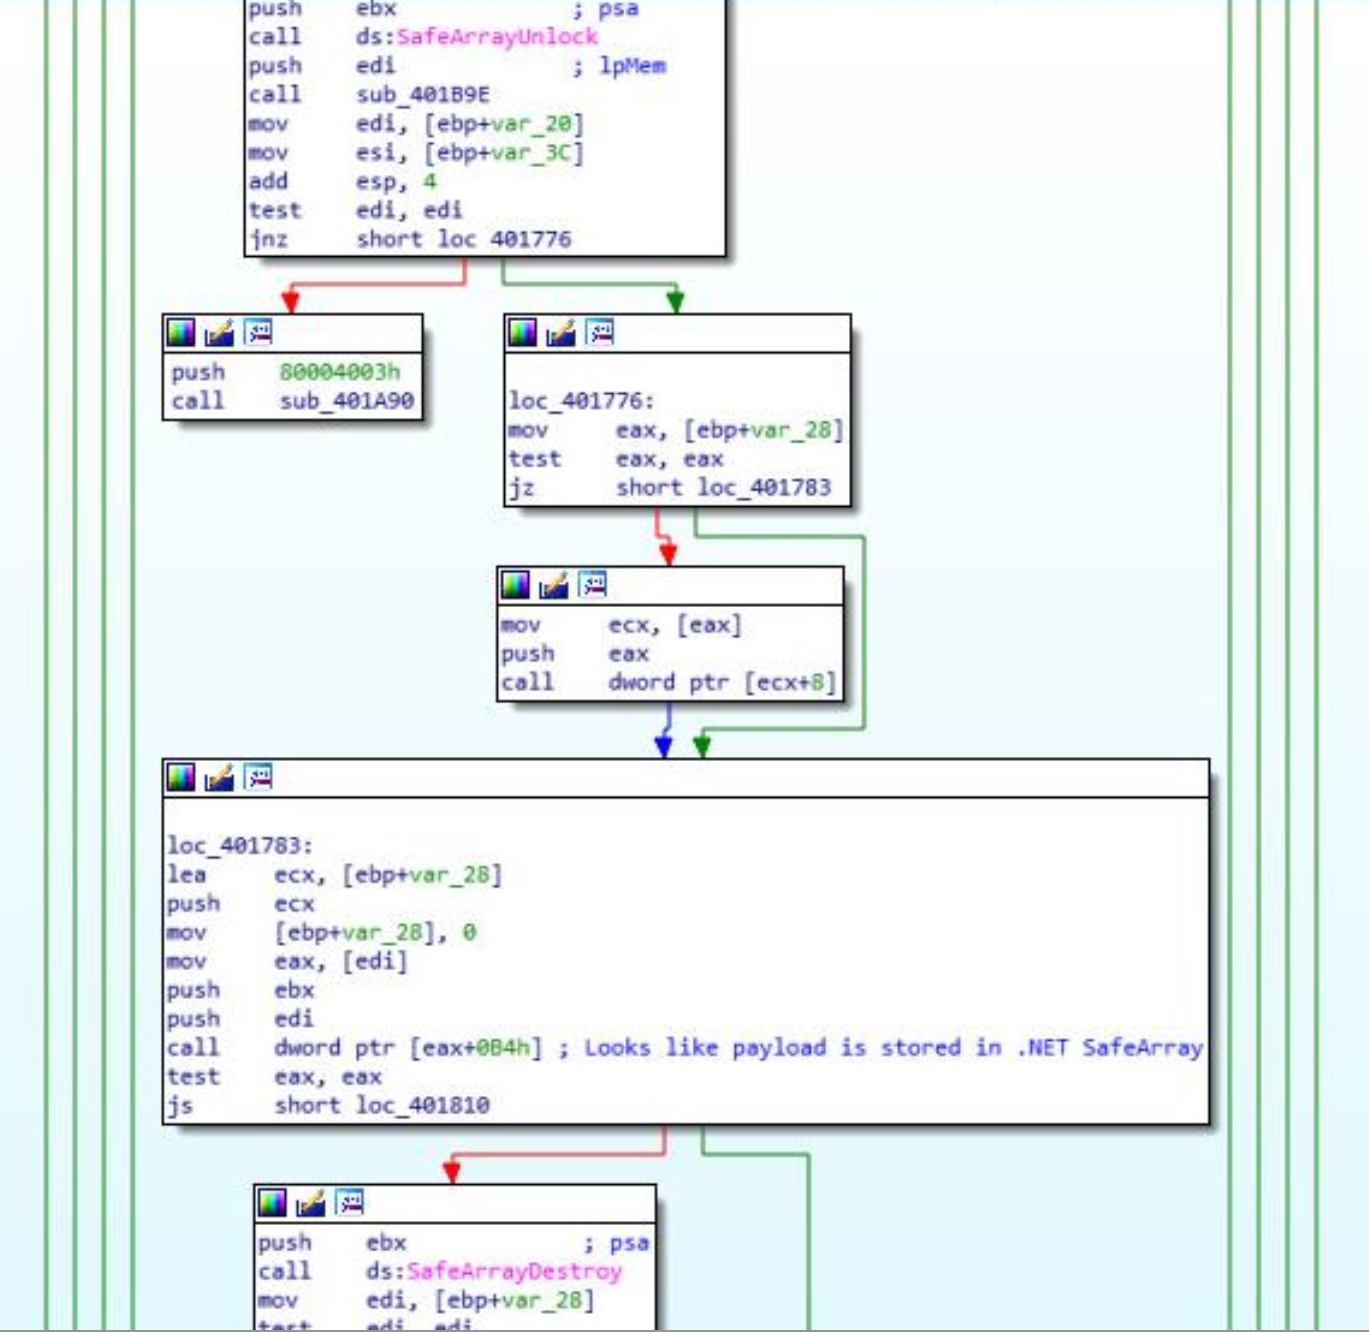
\includegraphics[scale=0.45]{fancy-bear-unpacking-3}
      \end{center}
    \end{column}
  \end{columns}
\end{frame}

\begin{frame}
  \frametitle{Unpacking Sofacy / FancyBear}
  \framesubtitle{solutions: 0x0e}
  \begin{center}
    \includegraphics[scale=0.45]{fancy-bear-unpacking-4}
  \end{center}
\end{frame}

\begin{frame}
  \frametitle{Unpacking Sofacy / FancyBear}
  \framesubtitle{solutions: 0x0e}
  \begin{columns}
    \begin{column}{.3\textwidth}
      \begin{itemize}
      \item{After Dumping the Data}
      \item{Interesting Metadata}
      \end{itemize}
    \end{column}
    \hfill
    \begin{column}{.7\textwidth}
      \begin{center}
        \includegraphics[scale=0.5]{fancy-bear-unpacking-5}
      \end{center}
    \end{column}
  \end{columns}
\end{frame}

\begin{frame}
  \frametitle{Unpacking Sofacy / FancyBear}
  \framesubtitle{solutions: 0x0e}
  \begin{center}
    \begin{figure}
      \includegraphics[scale=0.40]{fancy-bear-unpacking-6}
      \caption{Sofacy Dumped Payload - Appears Unpacked}
    \end{figure}
  \end{center}
  NOTE: Looks like this is in .NET so let's use DnSpy!
\end{frame}

\begin{frame}
  \frametitle{Unpacking Sofacy / FancyBear}
  \framesubtitle{solutions: 0x0e}
  \begin{center}
    \begin{figure}
      \includegraphics[scale=0.43]{fancy-bear-unpacking-7}
      \caption{Sofacy / FancyBear - CnC Code}
    \end{figure}
  \end{center}
\end{frame}

\begin{frame}
  \frametitle{Unpacking Stuxnet}
  \framesubtitle{solutions: 0x0f}
  \begin{center}
    Placeholder
  \end{center}
\end{frame}

\begin{frame}
  \frametitle{Unpacking KPot}
  \framesubtitle{solutions: 0x00}
  \begin{center}
    Placeholder
  \end{center}
\end{frame}

\begin{frame}
  \frametitle{References}
  \begin{center}
    Placeholder
  \end{center}
\end{frame}

\end{document}

% References
% https://en.wikibooks.org/wiki/X86_Disassembly/Calling_Conventions
% https://github.com/m0n0ph1/Process-Hollowing
% http://blog.sevagas.com/?PE-injection-explained
% https://en.wikipedia.org/wiki/DLL_injection